\chapter{The Deep Underground Neutrino Experiment}
\label{ch:dune}

The Deep Underground Neutrino Experiment (DUNE) is a long-baseline neutrino oscillation experiment currently under construction at two sites in the USA~\cite{tdrVol1, tdrVol2, tdrVol3, tdrVol4}.
The near detector site which will host the beam production facilities and the multi-component near detector is located at Fermilab, Illinois while the far detector site will be located at Sanford Underground Research Facility (SURF), South Dakota.
This will provide a baseline of approximately 1300~km.
A cartoon showing the arrangement of the detectors is shown in \citefig{fig:duneCartoon}.

\begin{figure}[h]
  \centering
  \includegraphics[width=.9\linewidth]{files/figures/dune_detector/duneCartoon}
  \caption[Cartoon of DUNE.]{Cartoon showing the arrangement of DUNE (not to scale) with the neutrino beam propagating from Fermilab to SURF along its 1300~km baseline. Taken from~\cite{tdrVol1}.}
  \label{fig:duneCartoon}
\end{figure}

In this chapter, the DUNE detector will be discussed.
Section~\ref{sec:dune:overview} will provide an overview of the detector, its motivation and its physics goals.
Section~\ref{sec:dune:fd} will discuss the design of the far detector.
Section~\ref{sec:dune:nd} will discuss the design of the near detector and Section~\ref{sec:dune:beam} will discuss the design of the beam.

\section{Overview and physics goals}
\label{sec:dune:overview}
As discussed in Section~\ref{sec:theory:currentState}, several questions remain in the field of neutrino oscillations.
Namely, the ordering of the neutrino mass eigenstates is not yet known and the value of $\delta_{CP}$ in the PMNS matrix remains unknown, which could imply that neutrinos violate Charge-Parity symmetry if it is proven that $\delta_{CP} \neq 0, \pi$.
Additionally, DUNE aims to be able to resolve the octant of $\theta_{23}$ (i.e. is $\theta_{23} > \pi/4$ or $< \pi/4$?) and usher in a new era of precision measurements of the PMNS matrix. 
DUNE aims to answer these questions, among others.

Due to the large volume of the far detector, it is also designed to observe neutrinos from a galactic core-collapse supernova if one should occur during the running time of the experiments.
This same large far detector mass will also allow it to search for certain Beyond the Standard Model (BSM) processes such as baryon number violation via proton decay.
A range of other BSM processes will also be explored by the experiment.

% Physics goals
% Oscillations first and foremost are the most important - refer to what is in the historical context chapter
DUNE aims to achieve its oscillation physics goals by simultaneously measuring the rates of $\nu_{\mu}$, $\bar{\nu}_{\mu}$, $\nu_{e}$ and $\bar{\nu}_{e}$ interactions in the near and far detectors as a function of neutrino energy.
From these measurements, the values of various oscillation parameters can be determined (see \citesec{sec:theory:theory:threeNeutrino} for further details on three neutrino oscillations). 
Enhanced fluxes of $\bar{\nu}_{\mu}$ and $\bar{\nu}_{e}$ are achieved by changing the polarity of the focussing horns used to produced the beam (see Section~\ref{sec:dune:beam} for details).
In terms of terminology, the enhanced neutrino beam is produced using the Forward Horn Current (FHC) polarity while the the enhanced antineutrino beam is produced using the Reverse Horn Current (RHC) polarity.

DUNE's proposed oscillation physics milestones are shown in \citetab{tab:physicsMilestones} along with their estimated expected running times.
DUNE's ability to meet these goals depends on several factors.

Firstly, DUNE will on the large number of neutrino interactions it will be able to observe.
These high statistics derive from the large fiducial mass of the far detector (40~kt eventually) and the high beam power (1.2~MW initially with later planned upgrades to 2.4~MW).

The far detector will consist of four liquid argon time projection chambers (LArTPCs).
These modules will combine excellent particle identification and energy resolution will a large, monolithic detector mass. 
The operation principles of LArTPCs will be discussed further in \citesec{sec:dune:fd:lartpc}.
\citetab{tab:statistics} shows the number of expected neutrino interactions in the far detector for 3.5 years of staged running.

\begin{table}
  \caption[DUNE oscillation physics milestones.]{Table from~\cite{tdrVol2} showing the expected DUNE oscillation physics milestones and their required exposure in years, assuming the true neutrino mass hierarchy is normally ordered and equal running in with both forward and reverse horn currents. The best fit parameters in~\cite{nufit4} are used.}
  \label{tab:physicsMilestones}
  \centering
  \begin{tabular}{c c}
    \hline
    Physics milestone & Exposure (staged years) \\
    \hline
    $5\sigma$ mass ordering ($\delta_{CP} = -\pi/2$) & 1 \\
    $5\sigma$ mass ordering (all $\delta_{CP}$ values) & 2 \\
    $3\sigma$ CP violation ($\delta_{CP}=-\pi/2$) & 3 \\
    $3\sigma$ CP violation (50\% of $\delta_{CP}$ values) & 5 \\
    $5\sigma$ CP violation ($\delta_{CP}=-\pi/2$) & 7 \\
    $5\sigma$ CP violation (50\% of $\delta_{CP}$ values) & 10 \\
    $3\sigma$ CP violation (75\% of $\delta_{CP}$ values) & 13 \\
    $\delta_{CP}$ resolution of $10^{\circ}$ ($\delta_{CP}=0$) & 8 \\
    $\delta_{CP}$ resolution of $20^{\circ}$ ($\delta_{CP}=-\pi/2$) & 12 \\
    $\text{sin}^{2}2\theta_{13}$ resolution of 0.004 & 15 \\
    \hline
  \end{tabular}
\end{table}

\begin{table}
  \caption[Expected numbers of DUNE far detector events.]{Expected numbers of signal events for the DUNE far detector in the neutrino energy range \SIrange{0.5}{8}{\giga\electronvolt} for 3.5 years of staged exposures for both FHC and RHC running. The rates shown assume the mass hierarchy is normally ordered, that $\delta_{CP}=0$ and that all other oscillation parameters are at their best fit points in~\cite{nufit4}. Taken from~\cite{tdrVol2}.}
  \label{tab:statistics}
  \centering
  \begin{tabular}{c c}
    \hline
    Signal & Expected events \\
    \hline
    \hline
    \multicolumn{2}{c}{Neutrino mode} \\
    $\nu_{\mu}$ & 6200 \\
    $\bar{\nu}_{\mu}$ & 389 \\
    $\nu_{e}$ & 1092 \\
    $\bar{\nu}_{e}$ & 18 \\
    \hline
    \multicolumn{2}{c}{Antineutrino mode} \\
    $\nu_{\mu}$ & 1129 \\
    $\bar{\nu}_{\mu}$ & 2303 \\
    $\nu_{e}$ & 76 \\
    $\bar{\nu}_{e}$ & 224 \\
    \hline
  \end{tabular}
\end{table}

Secondly, DUNE will use a neutrino beam with a wide spread of neutrino energies which, given the values of the mass splittings, will allow it cover both the first and second oscillation maxima.
It is helpful to measure multiple oscillation maxima because of degeneracies between the oscillation parameters.
This means that, for a given neutrino energy, multiple sets of parameter values can realise the same oscillation probability.

Some of the benefits of the broad band beam are shown in \citefig{fig:nueRates}.
\citefig{fig:nueRates} is a so-called `bi-rate' plot which shows the rates of \nue and \anue interactions at the far detector for various values of the oscillation parameters.
To make each of the ellipses, all oscillation parameters are held constant other than \dcp which is varied.
The blue (green) ellipses show the rates for the first (second) oscillation maximum.
The first oscillation maximum is defined as being at energies higher than the approximate first oscillation minimum at \SI{1.3}{\giga\electronvolt}, while the second oscillation maximum is defined as anything below this.
The solid (dashed) lines show the rates for the normal (inverted) neutrino mass hierarchy.
The red and black points highlight the maximally CP-violating cases.
Here, $\thetai{23}=\pi/4$ while the other mixing angles and mass splittings are at their best fit points according to~\cite{nufit4}.

\begin{figure}[h]
  \begin{minipage}[t]{0.49\textwidth}
    \begin{adjustbox}{max totalsize={\textwidth}, center}
      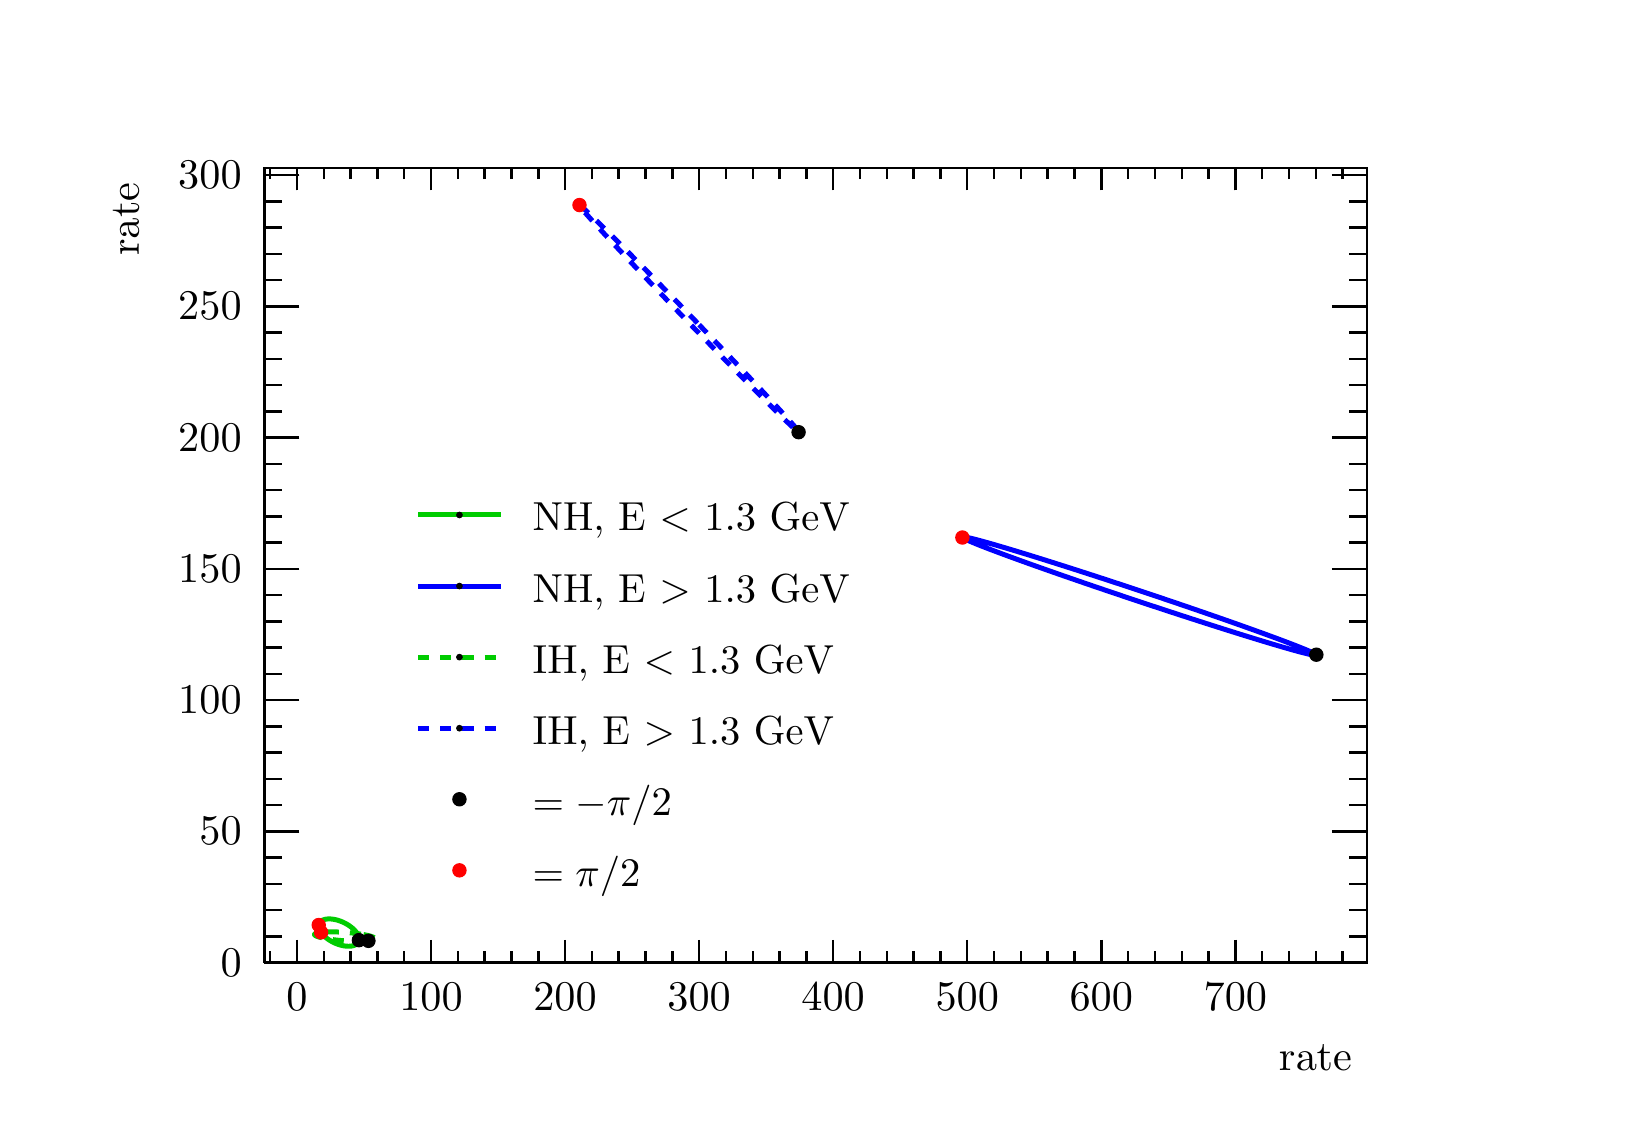
\begin{tikzpicture}
\pgfdeclareplotmark{cross} {
\pgfpathmoveto{\pgfpoint{-0.3\pgfplotmarksize}{\pgfplotmarksize}}
\pgfpathlineto{\pgfpoint{+0.3\pgfplotmarksize}{\pgfplotmarksize}}
\pgfpathlineto{\pgfpoint{+0.3\pgfplotmarksize}{0.3\pgfplotmarksize}}
\pgfpathlineto{\pgfpoint{+1\pgfplotmarksize}{0.3\pgfplotmarksize}}
\pgfpathlineto{\pgfpoint{+1\pgfplotmarksize}{-0.3\pgfplotmarksize}}
\pgfpathlineto{\pgfpoint{+0.3\pgfplotmarksize}{-0.3\pgfplotmarksize}}
\pgfpathlineto{\pgfpoint{+0.3\pgfplotmarksize}{-1.\pgfplotmarksize}}
\pgfpathlineto{\pgfpoint{-0.3\pgfplotmarksize}{-1.\pgfplotmarksize}}
\pgfpathlineto{\pgfpoint{-0.3\pgfplotmarksize}{-0.3\pgfplotmarksize}}
\pgfpathlineto{\pgfpoint{-1.\pgfplotmarksize}{-0.3\pgfplotmarksize}}
\pgfpathlineto{\pgfpoint{-1.\pgfplotmarksize}{0.3\pgfplotmarksize}}
\pgfpathlineto{\pgfpoint{-0.3\pgfplotmarksize}{0.3\pgfplotmarksize}}
\pgfpathclose
\pgfusepathqstroke
}
\pgfdeclareplotmark{cross*} {
\pgfpathmoveto{\pgfpoint{-0.3\pgfplotmarksize}{\pgfplotmarksize}}
\pgfpathlineto{\pgfpoint{+0.3\pgfplotmarksize}{\pgfplotmarksize}}
\pgfpathlineto{\pgfpoint{+0.3\pgfplotmarksize}{0.3\pgfplotmarksize}}
\pgfpathlineto{\pgfpoint{+1\pgfplotmarksize}{0.3\pgfplotmarksize}}
\pgfpathlineto{\pgfpoint{+1\pgfplotmarksize}{-0.3\pgfplotmarksize}}
\pgfpathlineto{\pgfpoint{+0.3\pgfplotmarksize}{-0.3\pgfplotmarksize}}
\pgfpathlineto{\pgfpoint{+0.3\pgfplotmarksize}{-1.\pgfplotmarksize}}
\pgfpathlineto{\pgfpoint{-0.3\pgfplotmarksize}{-1.\pgfplotmarksize}}
\pgfpathlineto{\pgfpoint{-0.3\pgfplotmarksize}{-0.3\pgfplotmarksize}}
\pgfpathlineto{\pgfpoint{-1.\pgfplotmarksize}{-0.3\pgfplotmarksize}}
\pgfpathlineto{\pgfpoint{-1.\pgfplotmarksize}{0.3\pgfplotmarksize}}
\pgfpathlineto{\pgfpoint{-0.3\pgfplotmarksize}{0.3\pgfplotmarksize}}
\pgfpathclose
\pgfusepathqfillstroke
}
\pgfdeclareplotmark{newstar} {
\pgfpathmoveto{\pgfqpoint{0pt}{\pgfplotmarksize}}
\pgfpathlineto{\pgfqpointpolar{44}{0.5\pgfplotmarksize}}
\pgfpathlineto{\pgfqpointpolar{18}{\pgfplotmarksize}}
\pgfpathlineto{\pgfqpointpolar{-20}{0.5\pgfplotmarksize}}
\pgfpathlineto{\pgfqpointpolar{-54}{\pgfplotmarksize}}
\pgfpathlineto{\pgfqpointpolar{-90}{0.5\pgfplotmarksize}}
\pgfpathlineto{\pgfqpointpolar{234}{\pgfplotmarksize}}
\pgfpathlineto{\pgfqpointpolar{198}{0.5\pgfplotmarksize}}
\pgfpathlineto{\pgfqpointpolar{162}{\pgfplotmarksize}}
\pgfpathlineto{\pgfqpointpolar{134}{0.5\pgfplotmarksize}}
\pgfpathclose
\pgfusepathqstroke
}
\pgfdeclareplotmark{newstar*} {
\pgfpathmoveto{\pgfqpoint{0pt}{\pgfplotmarksize}}
\pgfpathlineto{\pgfqpointpolar{44}{0.5\pgfplotmarksize}}
\pgfpathlineto{\pgfqpointpolar{18}{\pgfplotmarksize}}
\pgfpathlineto{\pgfqpointpolar{-20}{0.5\pgfplotmarksize}}
\pgfpathlineto{\pgfqpointpolar{-54}{\pgfplotmarksize}}
\pgfpathlineto{\pgfqpointpolar{-90}{0.5\pgfplotmarksize}}
\pgfpathlineto{\pgfqpointpolar{234}{\pgfplotmarksize}}
\pgfpathlineto{\pgfqpointpolar{198}{0.5\pgfplotmarksize}}
\pgfpathlineto{\pgfqpointpolar{162}{\pgfplotmarksize}}
\pgfpathlineto{\pgfqpointpolar{134}{0.5\pgfplotmarksize}}
\pgfpathclose
\pgfusepathqfillstroke
}
\definecolor{c}{rgb}{1,1,1};
\draw [color=c, fill=c] (0,0) rectangle (20,13.639);
\draw [color=c, fill=c] (3,1.77307) rectangle (17,11.8659);
\definecolor{c}{rgb}{0,0,0};
\draw [c,line width=0.9] (3,1.77307) -- (3,11.8659) -- (17,11.8659) -- (17,1.77307) -- (3,1.77307);
\definecolor{c}{rgb}{1,1,1};
\draw [color=c, fill=c] (3,1.77307) rectangle (17,11.8659);
\definecolor{c}{rgb}{0,0,0};
\draw [c,line width=0.9] (3,1.77307) -- (3,11.8659) -- (17,11.8659) -- (17,1.77307) -- (3,1.77307);
\draw [c,line width=0.9] (3,1.77307) -- (17,1.77307);
\draw [c,line width=0.9] (3.41282,2.05948) -- (3.41282,1.77307);
\draw [c,line width=0.9] (3.75333,1.91628) -- (3.75333,1.77307);
\draw [c,line width=0.9] (4.09383,1.91628) -- (4.09383,1.77307);
\draw [c,line width=0.9] (4.43433,1.91628) -- (4.43433,1.77307);
\draw [c,line width=0.9] (4.77484,1.91628) -- (4.77484,1.77307);
\draw [c,line width=0.9] (5.11534,2.05948) -- (5.11534,1.77307);
\draw [c,line width=0.9] (5.45585,1.91628) -- (5.45585,1.77307);
\draw [c,line width=0.9] (5.79635,1.91628) -- (5.79635,1.77307);
\draw [c,line width=0.9] (6.13686,1.91628) -- (6.13686,1.77307);
\draw [c,line width=0.9] (6.47736,1.91628) -- (6.47736,1.77307);
\draw [c,line width=0.9] (6.81786,2.05948) -- (6.81786,1.77307);
\draw [c,line width=0.9] (7.15837,1.91628) -- (7.15837,1.77307);
\draw [c,line width=0.9] (7.49887,1.91628) -- (7.49887,1.77307);
\draw [c,line width=0.9] (7.83938,1.91628) -- (7.83938,1.77307);
\draw [c,line width=0.9] (8.17988,1.91628) -- (8.17988,1.77307);
\draw [c,line width=0.9] (8.52039,2.05948) -- (8.52039,1.77307);
\draw [c,line width=0.9] (8.86089,1.91628) -- (8.86089,1.77307);
\draw [c,line width=0.9] (9.20139,1.91628) -- (9.20139,1.77307);
\draw [c,line width=0.9] (9.5419,1.91628) -- (9.5419,1.77307);
\draw [c,line width=0.9] (9.8824,1.91628) -- (9.8824,1.77307);
\draw [c,line width=0.9] (10.2229,2.05948) -- (10.2229,1.77307);
\draw [c,line width=0.9] (10.5634,1.91628) -- (10.5634,1.77307);
\draw [c,line width=0.9] (10.9039,1.91628) -- (10.9039,1.77307);
\draw [c,line width=0.9] (11.2444,1.91628) -- (11.2444,1.77307);
\draw [c,line width=0.9] (11.5849,1.91628) -- (11.5849,1.77307);
\draw [c,line width=0.9] (11.9254,2.05948) -- (11.9254,1.77307);
\draw [c,line width=0.9] (12.2659,1.91628) -- (12.2659,1.77307);
\draw [c,line width=0.9] (12.6064,1.91628) -- (12.6064,1.77307);
\draw [c,line width=0.9] (12.9469,1.91628) -- (12.9469,1.77307);
\draw [c,line width=0.9] (13.2874,1.91628) -- (13.2874,1.77307);
\draw [c,line width=0.9] (13.628,2.05948) -- (13.628,1.77307);
\draw [c,line width=0.9] (13.9685,1.91628) -- (13.9685,1.77307);
\draw [c,line width=0.9] (14.309,1.91628) -- (14.309,1.77307);
\draw [c,line width=0.9] (14.6495,1.91628) -- (14.6495,1.77307);
\draw [c,line width=0.9] (14.99,1.91628) -- (14.99,1.77307);
\draw [c,line width=0.9] (15.3305,2.05948) -- (15.3305,1.77307);
\draw [c,line width=0.9] (3.41282,2.05948) -- (3.41282,1.77307);
\draw [c,line width=0.9] (3.07232,1.91628) -- (3.07232,1.77307);
\draw [c,line width=0.9] (15.3305,2.05948) -- (15.3305,1.77307);
\draw [c,line width=0.9] (15.671,1.91628) -- (15.671,1.77307);
\draw [c,line width=0.9] (16.0115,1.91628) -- (16.0115,1.77307);
\draw [c,line width=0.9] (16.352,1.91628) -- (16.352,1.77307);
\draw [c,line width=0.9] (16.6925,1.91628) -- (16.6925,1.77307);
\draw [anchor=base] (3.41282,1.15931) node[scale=1.52731, color=c, rotate=0]{0};
\draw [anchor=base] (5.11534,1.15931) node[scale=1.52731, color=c, rotate=0]{100};
\draw [anchor=base] (6.81786,1.15931) node[scale=1.52731, color=c, rotate=0]{200};
\draw [anchor=base] (8.52039,1.15931) node[scale=1.52731, color=c, rotate=0]{300};
\draw [anchor=base] (10.2229,1.15931) node[scale=1.52731, color=c, rotate=0]{400};
\draw [anchor=base] (11.9254,1.15931) node[scale=1.52731, color=c, rotate=0]{500};
\draw [anchor=base] (13.628,1.15931) node[scale=1.52731, color=c, rotate=0]{600};
\draw [anchor=base] (15.3305,1.15931) node[scale=1.52731, color=c, rotate=0]{700};
\draw [anchor= east] (17,0.572837) node[scale=1.52731, color=c, rotate=0]{\nue rate};
\draw [c,line width=0.9] (3,11.8659) -- (17,11.8659);
\draw [c,line width=0.9] (3.41282,11.5795) -- (3.41282,11.8659);
\draw [c,line width=0.9] (3.75333,11.7227) -- (3.75333,11.8659);
\draw [c,line width=0.9] (4.09383,11.7227) -- (4.09383,11.8659);
\draw [c,line width=0.9] (4.43433,11.7227) -- (4.43433,11.8659);
\draw [c,line width=0.9] (4.77484,11.7227) -- (4.77484,11.8659);
\draw [c,line width=0.9] (5.11534,11.5795) -- (5.11534,11.8659);
\draw [c,line width=0.9] (5.45585,11.7227) -- (5.45585,11.8659);
\draw [c,line width=0.9] (5.79635,11.7227) -- (5.79635,11.8659);
\draw [c,line width=0.9] (6.13686,11.7227) -- (6.13686,11.8659);
\draw [c,line width=0.9] (6.47736,11.7227) -- (6.47736,11.8659);
\draw [c,line width=0.9] (6.81786,11.5795) -- (6.81786,11.8659);
\draw [c,line width=0.9] (7.15837,11.7227) -- (7.15837,11.8659);
\draw [c,line width=0.9] (7.49887,11.7227) -- (7.49887,11.8659);
\draw [c,line width=0.9] (7.83938,11.7227) -- (7.83938,11.8659);
\draw [c,line width=0.9] (8.17988,11.7227) -- (8.17988,11.8659);
\draw [c,line width=0.9] (8.52039,11.5795) -- (8.52039,11.8659);
\draw [c,line width=0.9] (8.86089,11.7227) -- (8.86089,11.8659);
\draw [c,line width=0.9] (9.20139,11.7227) -- (9.20139,11.8659);
\draw [c,line width=0.9] (9.5419,11.7227) -- (9.5419,11.8659);
\draw [c,line width=0.9] (9.8824,11.7227) -- (9.8824,11.8659);
\draw [c,line width=0.9] (10.2229,11.5795) -- (10.2229,11.8659);
\draw [c,line width=0.9] (10.5634,11.7227) -- (10.5634,11.8659);
\draw [c,line width=0.9] (10.9039,11.7227) -- (10.9039,11.8659);
\draw [c,line width=0.9] (11.2444,11.7227) -- (11.2444,11.8659);
\draw [c,line width=0.9] (11.5849,11.7227) -- (11.5849,11.8659);
\draw [c,line width=0.9] (11.9254,11.5795) -- (11.9254,11.8659);
\draw [c,line width=0.9] (12.2659,11.7227) -- (12.2659,11.8659);
\draw [c,line width=0.9] (12.6064,11.7227) -- (12.6064,11.8659);
\draw [c,line width=0.9] (12.9469,11.7227) -- (12.9469,11.8659);
\draw [c,line width=0.9] (13.2874,11.7227) -- (13.2874,11.8659);
\draw [c,line width=0.9] (13.628,11.5795) -- (13.628,11.8659);
\draw [c,line width=0.9] (13.9685,11.7227) -- (13.9685,11.8659);
\draw [c,line width=0.9] (14.309,11.7227) -- (14.309,11.8659);
\draw [c,line width=0.9] (14.6495,11.7227) -- (14.6495,11.8659);
\draw [c,line width=0.9] (14.99,11.7227) -- (14.99,11.8659);
\draw [c,line width=0.9] (15.3305,11.5795) -- (15.3305,11.8659);
\draw [c,line width=0.9] (3.41282,11.5795) -- (3.41282,11.8659);
\draw [c,line width=0.9] (3.07232,11.7227) -- (3.07232,11.8659);
\draw [c,line width=0.9] (15.3305,11.5795) -- (15.3305,11.8659);
\draw [c,line width=0.9] (15.671,11.7227) -- (15.671,11.8659);
\draw [c,line width=0.9] (16.0115,11.7227) -- (16.0115,11.8659);
\draw [c,line width=0.9] (16.352,11.7227) -- (16.352,11.8659);
\draw [c,line width=0.9] (16.6925,11.7227) -- (16.6925,11.8659);
\draw [c,line width=0.9] (3,1.77307) -- (3,11.8659);
\draw [c,line width=0.9] (3.444,1.77307) -- (3,1.77307);
\draw [c,line width=0.9] (3.222,2.10645) -- (3,2.10645);
\draw [c,line width=0.9] (3.222,2.43983) -- (3,2.43983);
\draw [c,line width=0.9] (3.222,2.77321) -- (3,2.77321);
\draw [c,line width=0.9] (3.222,3.10659) -- (3,3.10659);
\draw [c,line width=0.9] (3.444,3.43997) -- (3,3.43997);
\draw [c,line width=0.9] (3.222,3.77335) -- (3,3.77335);
\draw [c,line width=0.9] (3.222,4.10674) -- (3,4.10674);
\draw [c,line width=0.9] (3.222,4.44012) -- (3,4.44012);
\draw [c,line width=0.9] (3.222,4.7735) -- (3,4.7735);
\draw [c,line width=0.9] (3.444,5.10688) -- (3,5.10688);
\draw [c,line width=0.9] (3.222,5.44026) -- (3,5.44026);
\draw [c,line width=0.9] (3.222,5.77364) -- (3,5.77364);
\draw [c,line width=0.9] (3.222,6.10702) -- (3,6.10702);
\draw [c,line width=0.9] (3.222,6.4404) -- (3,6.4404);
\draw [c,line width=0.9] (3.444,6.77379) -- (3,6.77379);
\draw [c,line width=0.9] (3.222,7.10717) -- (3,7.10717);
\draw [c,line width=0.9] (3.222,7.44055) -- (3,7.44055);
\draw [c,line width=0.9] (3.222,7.77393) -- (3,7.77393);
\draw [c,line width=0.9] (3.222,8.10731) -- (3,8.10731);
\draw [c,line width=0.9] (3.444,8.44069) -- (3,8.44069);
\draw [c,line width=0.9] (3.222,8.77407) -- (3,8.77407);
\draw [c,line width=0.9] (3.222,9.10746) -- (3,9.10746);
\draw [c,line width=0.9] (3.222,9.44084) -- (3,9.44084);
\draw [c,line width=0.9] (3.222,9.77422) -- (3,9.77422);
\draw [c,line width=0.9] (3.444,10.1076) -- (3,10.1076);
\draw [c,line width=0.9] (3.222,10.441) -- (3,10.441);
\draw [c,line width=0.9] (3.222,10.7744) -- (3,10.7744);
\draw [c,line width=0.9] (3.222,11.1077) -- (3,11.1077);
\draw [c,line width=0.9] (3.222,11.4411) -- (3,11.4411);
\draw [c,line width=0.9] (3.444,11.7745) -- (3,11.7745);
\draw [c,line width=0.9] (3.444,11.7745) -- (3,11.7745);
\draw [anchor= east] (2.9,1.77307) node[scale=1.52731, color=c, rotate=0]{0};
\draw [anchor= east] (2.9,3.43997) node[scale=1.52731, color=c, rotate=0]{50};
\draw [anchor= east] (2.9,5.10688) node[scale=1.52731, color=c, rotate=0]{100};
\draw [anchor= east] (2.9,6.77379) node[scale=1.52731, color=c, rotate=0]{150};
\draw [anchor= east] (2.9,8.44069) node[scale=1.52731, color=c, rotate=0]{200};
\draw [anchor= east] (2.9,10.1076) node[scale=1.52731, color=c, rotate=0]{250};
\draw [anchor= east] (2.9,11.7745) node[scale=1.52731, color=c, rotate=0]{300};
\draw [anchor= east] (1.24,11.8659) node[scale=1.52731, color=c, rotate=90]{\anue rate};
\draw [c,line width=0.9] (17,1.77307) -- (17,11.8659);
\draw [c,line width=0.9] (16.556,1.77307) -- (17,1.77307);
\draw [c,line width=0.9] (16.778,2.10645) -- (17,2.10645);
\draw [c,line width=0.9] (16.778,2.43983) -- (17,2.43983);
\draw [c,line width=0.9] (16.778,2.77321) -- (17,2.77321);
\draw [c,line width=0.9] (16.778,3.10659) -- (17,3.10659);
\draw [c,line width=0.9] (16.556,3.43997) -- (17,3.43997);
\draw [c,line width=0.9] (16.778,3.77335) -- (17,3.77335);
\draw [c,line width=0.9] (16.778,4.10674) -- (17,4.10674);
\draw [c,line width=0.9] (16.778,4.44012) -- (17,4.44012);
\draw [c,line width=0.9] (16.778,4.7735) -- (17,4.7735);
\draw [c,line width=0.9] (16.556,5.10688) -- (17,5.10688);
\draw [c,line width=0.9] (16.778,5.44026) -- (17,5.44026);
\draw [c,line width=0.9] (16.778,5.77364) -- (17,5.77364);
\draw [c,line width=0.9] (16.778,6.10702) -- (17,6.10702);
\draw [c,line width=0.9] (16.778,6.4404) -- (17,6.4404);
\draw [c,line width=0.9] (16.556,6.77379) -- (17,6.77379);
\draw [c,line width=0.9] (16.778,7.10717) -- (17,7.10717);
\draw [c,line width=0.9] (16.778,7.44055) -- (17,7.44055);
\draw [c,line width=0.9] (16.778,7.77393) -- (17,7.77393);
\draw [c,line width=0.9] (16.778,8.10731) -- (17,8.10731);
\draw [c,line width=0.9] (16.556,8.44069) -- (17,8.44069);
\draw [c,line width=0.9] (16.778,8.77407) -- (17,8.77407);
\draw [c,line width=0.9] (16.778,9.10746) -- (17,9.10746);
\draw [c,line width=0.9] (16.778,9.44084) -- (17,9.44084);
\draw [c,line width=0.9] (16.778,9.77422) -- (17,9.77422);
\draw [c,line width=0.9] (16.556,10.1076) -- (17,10.1076);
\draw [c,line width=0.9] (16.778,10.441) -- (17,10.441);
\draw [c,line width=0.9] (16.778,10.7744) -- (17,10.7744);
\draw [c,line width=0.9] (16.778,11.1077) -- (17,11.1077);
\draw [c,line width=0.9] (16.778,11.4411) -- (17,11.4411);
\draw [c,line width=0.9] (16.556,11.7745) -- (17,11.7745);
\draw [c,line width=0.9] (16.556,11.7745) -- (17,11.7745);
\definecolor{c}{rgb}{0,0.8,0};
\draw [c,line width=1.8] (3.92242,2.00908) -- (3.93044,2.00613) -- (3.93848,2.00333) -- (3.94652,2.00067) -- (3.95456,1.99817) -- (3.96259,1.99582) -- (3.9706,1.99363) -- (3.97859,1.99159) -- (3.98654,1.98971) -- (3.99446,1.988) -- (4.00232,1.98645)
 -- (4.01012,1.98506) -- (4.01786,1.98384) -- (4.02553,1.98279) -- (4.03312,1.9819) -- (4.04062,1.98119) -- (4.04803,1.98064) -- (4.05533,1.98027) -- (4.06252,1.98006) -- (4.0696,1.98003) -- (4.07656,1.98017) -- (4.08338,1.98048) -- (4.09007,1.98097)
 -- (4.09661,1.98162) -- (4.103,1.98244) -- (4.10924,1.98343) -- (4.11532,1.98459) -- (4.12122,1.98591) -- (4.12695,1.98741) -- (4.13251,1.98906) -- (4.13787,1.99088) -- (4.14305,1.99286) -- (4.14803,1.99499) -- (4.1528,1.99729) -- (4.15738,1.99973)
 -- (4.16174,2.00233) -- (4.16589,2.00508) -- (4.16982,2.00798) -- (4.17353,2.01102) -- (4.17701,2.0142) -- (4.18026,2.01751) -- (4.18328,2.02096) -- (4.18606,2.02455) -- (4.18861,2.02826) -- (4.19091,2.03209) -- (4.19298,2.03604) --
 (4.19479,2.04011) -- (4.19636,2.0443) -- (4.19768,2.04858) -- (4.19875,2.05298) -- (4.19957,2.05747) -- (4.20014,2.06206) -- (4.20046,2.06674) -- (4.20052,2.0715) -- (4.20033,2.07634) -- (4.19989,2.08126) -- (4.1992,2.08626) -- (4.19825,2.09131) --
 (4.19706,2.09643) -- (4.19561,2.10161) -- (4.19392,2.10684) -- (4.19198,2.11211) -- (4.1898,2.11743) -- (4.18737,2.12278) -- (4.18471,2.12816) -- (4.18181,2.13356) -- (4.17867,2.13899) -- (4.17531,2.14443) -- (4.17171,2.14988) -- (4.16789,2.15533)
 -- (4.16386,2.16079) -- (4.1596,2.16623) -- (4.15513,2.17166) -- (4.15046,2.17708) -- (4.14558,2.18247) -- (4.1405,2.18783) -- (4.13523,2.19316) -- (4.12977,2.19845) -- (4.12413,2.20369) -- (4.11831,2.20889) -- (4.11232,2.21403) -- (4.10616,2.21911)
 -- (4.09985,2.22413) -- (4.09338,2.22908) -- (4.08676,2.23395) -- (4.08001,2.23874) -- (4.07312,2.24345) -- (4.0661,2.24807) -- (4.05897,2.2526) -- (4.05172,2.25703) -- (4.04436,2.26136) -- (4.03691,2.26558) -- (4.02936,2.26969) -- (4.02173,2.27369)
 -- (4.01403,2.27757) -- (4.00625,2.28132) -- (3.99842,2.28495) -- (3.99053,2.28845) -- (3.9826,2.29182) -- (3.97463,2.29505) -- (3.96663,2.29814) -- (3.95861,2.30109) -- (3.95057,2.3039) -- (3.94253,2.30655) -- (3.93449,2.30905) -- (3.92646,2.3114)
 -- (3.91845,2.3136) -- (3.91046,2.31564) -- (3.90251,2.31751) -- (3.89459,2.31923) -- (3.88673,2.32078) -- (3.87893,2.32217) -- (3.87119,2.32339) -- (3.86352,2.32444) -- (3.85593,2.32532) -- (3.84843,2.32604) -- (3.84102,2.32658) --
 (3.83372,2.32696) -- (3.82653,2.32716) -- (3.81945,2.32719) -- (3.81249,2.32705) -- (3.80567,2.32674) -- (3.79898,2.32626) -- (3.79244,2.32561) -- (3.78605,2.32478) -- (3.77981,2.32379) -- (3.77373,2.32264) -- (3.76783,2.32131) -- (3.7621,2.31982)
 -- (3.75655,2.31816) -- (3.75118,2.31635) -- (3.746,2.31437) -- (3.74102,2.31223) -- (3.73625,2.30994) -- (3.73167,2.30749) -- (3.72731,2.30489) -- (3.72316,2.30214) -- (3.71923,2.29925) -- (3.71552,2.29621) -- (3.71204,2.29303) -- (3.70879,2.28971)
 -- (3.70577,2.28626) -- (3.70299,2.28268) -- (3.70044,2.27897) -- (3.69814,2.27513) -- (3.69608,2.27118) -- (3.69426,2.26711) -- (3.69269,2.26293) -- (3.69137,2.25864) -- (3.6903,2.25425) -- (3.68948,2.24975) -- (3.68891,2.24517) --
 (3.68859,2.24049) -- (3.68853,2.23573) -- (3.68872,2.23088) -- (3.68916,2.22596) -- (3.68985,2.22097) -- (3.6908,2.21591) -- (3.69199,2.21079) -- (3.69344,2.20561) -- (3.69513,2.20039) -- (3.69707,2.19511) -- (3.69925,2.1898) -- (3.70168,2.18445) --
 (3.70434,2.17907) -- (3.70724,2.17366) -- (3.71038,2.16823) -- (3.71374,2.16279) -- (3.71734,2.15734) -- (3.72116,2.15189) -- (3.7252,2.14644) -- (3.72945,2.141) -- (3.73392,2.13556) -- (3.73859,2.13015) -- (3.74347,2.12476) -- (3.74855,2.1194) --
 (3.75382,2.11407) -- (3.75928,2.10878) -- (3.76492,2.10353) -- (3.77074,2.09834) -- (3.77673,2.09319) -- (3.78289,2.08811) -- (3.7892,2.0831) -- (3.79567,2.07815) -- (3.80229,2.07328) -- (3.80904,2.06848) -- (3.81593,2.06377) -- (3.82295,2.05915) --
 (3.83009,2.05462) -- (3.83733,2.05019) -- (3.84469,2.04586) -- (3.85214,2.04164) -- (3.85969,2.03753) -- (3.86732,2.03353) -- (3.87502,2.02966) -- (3.8828,2.0259) -- (3.89063,2.02227) -- (3.89852,2.01877) -- (3.90645,2.0154) -- (3.91442,2.01217) --
 (3.92242,2.00908);
\definecolor{c}{rgb}{0,0,1};
\draw [c,line width=1.8] (14.256,6.30899) -- (14.3265,6.28567) -- (14.3969,6.26249) -- (14.4669,6.23948) -- (14.5366,6.21665) -- (14.6058,6.19402) -- (14.6746,6.17163) -- (14.7428,6.14949) -- (14.8104,6.12762) -- (14.8773,6.10605) --
 (14.9435,6.08479) -- (15.0088,6.06387) -- (15.0732,6.04331) -- (15.1367,6.02313) -- (15.1992,6.00335) -- (15.2606,5.98398) -- (15.3209,5.96505) -- (15.38,5.94658) -- (15.4378,5.92858) -- (15.4943,5.91107) -- (15.5495,5.89407) -- (15.6032,5.8776) --
 (15.6555,5.86167) -- (15.7062,5.8463) -- (15.7554,5.8315) -- (15.8029,5.81728) -- (15.8488,5.80367) -- (15.893,5.79067) -- (15.9354,5.77831) -- (15.976,5.76658) -- (16.0147,5.7555) -- (16.0516,5.74508) -- (16.0866,5.73534) -- (16.1196,5.72628) --
 (16.1506,5.71791) -- (16.1797,5.71025) -- (16.2066,5.70328) -- (16.2316,5.69704) -- (16.2544,5.69151) -- (16.2751,5.68671) -- (16.2937,5.68263) -- (16.3101,5.6793) -- (16.3243,5.6767) -- (16.3364,5.67484) -- (16.3463,5.67372) -- (16.3539,5.67335) --
 (16.3594,5.67372) -- (16.3626,5.67483) -- (16.3636,5.67668) -- (16.3624,5.67928) -- (16.359,5.68261) -- (16.3533,5.68668) -- (16.3455,5.69147) -- (16.3354,5.697) -- (16.3231,5.70324) -- (16.3087,5.7102) -- (16.2921,5.71786) -- (16.2733,5.72623) --
 (16.2524,5.73528) -- (16.2294,5.74502) -- (16.2043,5.75543) -- (16.1771,5.7665) -- (16.1479,5.77823) -- (16.1167,5.79059) -- (16.0835,5.80359) -- (16.0484,5.81719) -- (16.0113,5.8314) -- (15.9724,5.8462) -- (15.9316,5.86157) -- (15.8891,5.8775) --
 (15.8448,5.89397) -- (15.7987,5.91096) -- (15.751,5.92847) -- (15.7017,5.94646) -- (15.6509,5.96493) -- (15.5985,5.98386) -- (15.5446,6.00322) -- (15.4893,6.023) -- (15.4327,6.04318) -- (15.3747,6.06374) -- (15.3155,6.08466) -- (15.2552,6.10591) --
 (15.1936,6.12748) -- (15.1311,6.14935) -- (15.0675,6.17149) -- (15.003,6.19388) -- (14.9376,6.2165) -- (14.8713,6.23933) -- (14.8044,6.26234) -- (14.7367,6.28552) -- (14.6684,6.30884) -- (14.5996,6.33227) -- (14.5303,6.35579) -- (14.4606,6.37939) --
 (14.3905,6.40303) -- (14.3202,6.4267) -- (14.2497,6.45036) -- (14.179,6.47401) -- (14.1082,6.4976) -- (14.0375,6.52113) -- (13.9668,6.54456) -- (13.8963,6.56788) -- (13.826,6.59105) -- (13.756,6.61407) -- (13.6863,6.6369) -- (13.617,6.65952) --
 (13.5482,6.68192) -- (13.48,6.70406) -- (13.4124,6.72593) -- (13.3455,6.7475) -- (13.2794,6.76875) -- (13.214,6.78967) -- (13.1496,6.81023) -- (13.0861,6.83042) -- (13.0236,6.8502) -- (12.9622,6.86957) -- (12.9019,6.88849) -- (12.8429,6.90697) --
 (12.785,6.92497) -- (12.7285,6.94247) -- (12.6734,6.95947) -- (12.6196,6.97595) -- (12.5674,6.99188) -- (12.5166,7.00725) -- (12.4674,7.02205) -- (12.4199,7.03626) -- (12.374,7.04988) -- (12.3299,7.06287) -- (12.2875,7.07524) -- (12.2469,7.08697) --
 (12.2081,7.09805) -- (12.1712,7.10846) -- (12.1363,7.1182) -- (12.1032,7.12726) -- (12.0722,7.13563) -- (12.0432,7.1433) -- (12.0162,7.15026) -- (11.9913,7.15651) -- (11.9685,7.16204) -- (11.9477,7.16684) -- (11.9292,7.17091) -- (11.9127,7.17425) --
 (11.8985,7.17685) -- (11.8864,7.17871) -- (11.8766,7.17983) -- (11.8689,7.1802) -- (11.8634,7.17983) -- (11.8602,7.17872) -- (11.8592,7.17686) -- (11.8604,7.17427) -- (11.8638,7.17094) -- (11.8695,7.16687) -- (11.8774,7.16207) -- (11.8874,7.15655)
 -- (11.8997,7.15031) -- (11.9141,7.14335) -- (11.9308,7.13568) -- (11.9495,7.12732) -- (11.9704,7.11827) -- (11.9934,7.10853) -- (12.0185,7.09812) -- (12.0457,7.08704) -- (12.0749,7.07532) -- (12.1061,7.06295) -- (12.1393,7.04996) --
 (12.1745,7.03635) -- (12.2115,7.02214) -- (12.2504,7.00735) -- (12.2912,6.99198) -- (12.3338,6.97605) -- (12.3781,6.95958) -- (12.4241,6.94259) -- (12.4718,6.92508) -- (12.5211,6.90709) -- (12.572,6.88862) -- (12.6244,6.86969) -- (12.6783,6.85033)
 -- (12.7335,6.83054) -- (12.7902,6.81037) -- (12.8481,6.78981) -- (12.9073,6.76889) -- (12.9677,6.74764) -- (13.0292,6.72607) -- (13.0918,6.7042) -- (13.1553,6.68206) -- (13.2199,6.65967) -- (13.2853,6.63705) -- (13.3515,6.61422) -- (13.4185,6.5912)
 -- (13.4861,6.56803) -- (13.5544,6.54471) -- (13.6232,6.52128) -- (13.6925,6.49775) -- (13.7622,6.47416) -- (13.8323,6.45052) -- (13.9026,6.42685) -- (13.9732,6.40318) -- (14.0439,6.37954) -- (14.1146,6.35595) -- (14.1853,6.33242) --
 (14.256,6.30899);
\definecolor{c}{rgb}{0,0.8,0};
\draw [c,dash pattern=on 4.00pt off 4.00pt ,line width=1.8] (4.25881,2.12821) -- (4.26812,2.1265) -- (4.27719,2.12476) -- (4.28601,2.12301) -- (4.29457,2.12123) -- (4.30285,2.11943) -- (4.31086,2.11762) -- (4.31857,2.1158) -- (4.326,2.11396) --
 (4.33312,2.11211) -- (4.33993,2.11025) -- (4.34643,2.10838) -- (4.3526,2.10651) -- (4.35845,2.10463) -- (4.36396,2.10276) -- (4.36914,2.10088) -- (4.37396,2.099) -- (4.37844,2.09713) -- (4.38257,2.09527) -- (4.38634,2.09341) -- (4.38974,2.09156) --
 (4.39278,2.08972) -- (4.39546,2.08789) -- (4.39776,2.08608) -- (4.39969,2.08429) -- (4.40125,2.08251) -- (4.40243,2.08076) -- (4.40323,2.07902) -- (4.40365,2.07731) -- (4.4037,2.07562) -- (4.40336,2.07397) -- (4.40265,2.07234) -- (4.40156,2.07073)
 -- (4.4001,2.06917) -- (4.39826,2.06763) -- (4.39604,2.06613) -- (4.39346,2.06467) -- (4.3905,2.06324) -- (4.38718,2.06185) -- (4.3835,2.0605) -- (4.37946,2.0592) -- (4.37507,2.05793) -- (4.37032,2.05672) -- (4.36523,2.05554) -- (4.3598,2.05442) --
 (4.35403,2.05334) -- (4.34793,2.05231) -- (4.34151,2.05133) -- (4.33478,2.0504) -- (4.32773,2.04952) -- (4.32038,2.0487) -- (4.31273,2.04792) -- (4.30479,2.04721) -- (4.29657,2.04654) -- (4.28808,2.04594) -- (4.27933,2.04539) -- (4.27031,2.04489) --
 (4.26106,2.04446) -- (4.25156,2.04408) -- (4.24183,2.04375) -- (4.23189,2.04349) -- (4.22174,2.04329) -- (4.21139,2.04314) -- (4.20084,2.04305) -- (4.19013,2.04303) -- (4.17924,2.04306) -- (4.16819,2.04315) -- (4.157,2.04329) -- (4.14568,2.0435) --
 (4.13423,2.04377) -- (4.12267,2.04409) -- (4.111,2.04447) -- (4.09925,2.04491) -- (4.08742,2.04541) -- (4.07552,2.04596) -- (4.06357,2.04657) -- (4.05157,2.04724) -- (4.03954,2.04796) -- (4.0275,2.04873) -- (4.01544,2.04956) -- (4.0034,2.05044) --
 (3.99136,2.05137) -- (3.97936,2.05235) -- (3.96739,2.05339) -- (3.95548,2.05447) -- (3.94363,2.05559) -- (3.93186,2.05677) -- (3.92017,2.05799) -- (3.90859,2.05925) -- (3.89711,2.06056) -- (3.88575,2.06191) -- (3.87453,2.0633) -- (3.86345,2.06473)
 -- (3.85252,2.0662) -- (3.84176,2.0677) -- (3.83118,2.06924) -- (3.82078,2.07081) -- (3.81058,2.07241) -- (3.80058,2.07404) -- (3.79081,2.0757) -- (3.78125,2.07739) -- (3.77194,2.0791) -- (3.76287,2.08083) -- (3.75405,2.08259) -- (3.74549,2.08437)
 -- (3.73721,2.08616) -- (3.7292,2.08798) -- (3.72149,2.0898) -- (3.71406,2.09164) -- (3.70694,2.09349) -- (3.70013,2.09535) -- (3.69363,2.09722) -- (3.68746,2.09909) -- (3.68161,2.10096) -- (3.6761,2.10284) -- (3.67093,2.10472) -- (3.6661,2.10659)
 -- (3.66162,2.10847) -- (3.65749,2.11033) -- (3.65372,2.11219) -- (3.65032,2.11404) -- (3.64728,2.11588) -- (3.6446,2.11771) -- (3.6423,2.11952) -- (3.64037,2.12131) -- (3.63881,2.12309) -- (3.63763,2.12484) -- (3.63683,2.12658) -- (3.63641,2.12829)
 -- (3.63636,2.12997) -- (3.6367,2.13163) -- (3.63741,2.13326) -- (3.6385,2.13486) -- (3.63996,2.13643) -- (3.6418,2.13797) -- (3.64402,2.13947) -- (3.6466,2.14093) -- (3.64956,2.14236) -- (3.65288,2.14375) -- (3.65656,2.1451) -- (3.6606,2.1464) --
 (3.66499,2.14766) -- (3.66974,2.14888) -- (3.67483,2.15006) -- (3.68026,2.15118) -- (3.68603,2.15226) -- (3.69213,2.15329) -- (3.69855,2.15427) -- (3.70528,2.1552) -- (3.71233,2.15608) -- (3.71968,2.1569) -- (3.72733,2.15767) -- (3.73527,2.15839) --
 (3.74349,2.15905) -- (3.75198,2.15966) -- (3.76074,2.16021) -- (3.76975,2.16071) -- (3.77901,2.16114) -- (3.7885,2.16152) -- (3.79823,2.16184) -- (3.80817,2.16211) -- (3.81832,2.16231) -- (3.82868,2.16246) -- (3.83922,2.16254) -- (3.84994,2.16257)
 -- (3.86082,2.16254) -- (3.87187,2.16245) -- (3.88306,2.1623) -- (3.89438,2.1621) -- (3.90583,2.16183) -- (3.91739,2.16151) -- (3.92906,2.16112) -- (3.94081,2.16068) -- (3.95264,2.16019) -- (3.96454,2.15963) -- (3.97649,2.15902) -- (3.98849,2.15836)
 -- (4.00052,2.15764) -- (4.01256,2.15687) -- (4.02462,2.15604) -- (4.03667,2.15516) -- (4.0487,2.15423) -- (4.0607,2.15324) -- (4.07267,2.15221) -- (4.08458,2.15113) -- (4.09643,2.15) -- (4.1082,2.14883) -- (4.11989,2.14761) -- (4.13147,2.14634) --
 (4.14295,2.14504) -- (4.15431,2.14369) -- (4.16553,2.1423) -- (4.17661,2.14087) -- (4.18754,2.1394) -- (4.1983,2.1379) -- (4.20888,2.13636) -- (4.21928,2.13479) -- (4.22948,2.13319) -- (4.23948,2.13156) -- (4.24925,2.1299) -- (4.25881,2.12821);
\definecolor{c}{rgb}{0,0,1};
\draw [c,dash pattern=on 4.00pt off 4.00pt ,line width=1.8] (8.52006,9.87307) -- (8.56369,9.82781) -- (8.60716,9.78266) -- (8.65042,9.73768) -- (8.69342,9.69292) -- (8.73612,9.6484) -- (8.77849,9.60419) -- (8.82047,9.56032) -- (8.86203,9.51683) --
 (8.90312,9.47377) -- (8.94372,9.43118) -- (8.98377,9.3891) -- (9.02323,9.34758) -- (9.06207,9.30666) -- (9.10025,9.26637) -- (9.13773,9.22675) -- (9.17448,9.18785) -- (9.21045,9.14971) -- (9.24562,9.11235) -- (9.27995,9.07582) -- (9.31339,9.04015)
 -- (9.34593,9.00539) -- (9.37753,8.97155) -- (9.40816,8.93869) -- (9.43778,8.90682) -- (9.46637,8.87598) -- (9.4939,8.8462) -- (9.52035,8.81751) -- (9.54568,8.78994) -- (9.56987,8.76352) -- (9.5929,8.73827) -- (9.61475,8.71421) -- (9.63539,8.69138)
 -- (9.6548,8.66979) -- (9.67297,8.64946) -- (9.68987,8.63042) -- (9.70549,8.61268) -- (9.71981,8.59626) -- (9.73283,8.58117) -- (9.74452,8.56744) -- (9.75488,8.55508) -- (9.76389,8.54409) -- (9.77155,8.53449) -- (9.77785,8.52629) --
 (9.78278,8.51949) -- (9.78634,8.5141) -- (9.78852,8.51014) -- (9.78933,8.50759) -- (9.78875,8.50647) -- (9.7868,8.50678) -- (9.78347,8.50851) -- (9.77877,8.51166) -- (9.7727,8.51624) -- (9.76527,8.52223) -- (9.75648,8.52962) -- (9.74635,8.53843) --
 (9.73488,8.54862) -- (9.72209,8.5602) -- (9.70798,8.57315) -- (9.69257,8.58747) -- (9.67588,8.60312) -- (9.65793,8.62011) -- (9.63872,8.63841) -- (9.61829,8.658) -- (9.59664,8.67888) -- (9.57381,8.701) -- (9.54981,8.72436) -- (9.52467,8.74893) --
 (9.49841,8.77469) -- (9.47106,8.80161) -- (9.44264,8.82966) -- (9.41319,8.85882) -- (9.38273,8.88905) -- (9.35129,8.92033) -- (9.31891,8.95263) -- (9.28561,8.98592) -- (9.25143,9.02016) -- (9.2164,9.05531) -- (9.18056,9.09135) -- (9.14394,9.12824)
 -- (9.10658,9.16594) -- (9.06851,9.20441) -- (9.02978,9.24362) -- (8.99041,9.28353) -- (8.95046,9.3241) -- (8.90996,9.36528) -- (8.86894,9.40705) -- (8.82746,9.44935) -- (8.78554,9.49214) -- (8.74324,9.53539) -- (8.70059,9.57905) --
 (8.65764,9.62307) -- (8.61442,9.66742) -- (8.57098,9.71205) -- (8.52737,9.75691) -- (8.48363,9.80197) -- (8.43979,9.84717) -- (8.39591,9.89247) -- (8.35203,9.93783) -- (8.30818,9.98321) -- (8.26442,10.0285) -- (8.22078,10.0738) -- (8.17731,10.119)
 -- (8.13406,10.1639) -- (8.09106,10.2087) -- (8.04835,10.2532) -- (8.00599,10.2974) -- (7.96401,10.3413) -- (7.92245,10.3848) -- (7.88135,10.4279) -- (7.84076,10.4704) -- (7.80071,10.5125) -- (7.76125,10.554) -- (7.7224,10.595) -- (7.68422,10.6353)
 -- (7.64674,10.6749) -- (7.61,10.7138) -- (7.57402,10.7519) -- (7.53885,10.7893) -- (7.50453,10.8258) -- (7.47108,10.8615) -- (7.43854,10.8962) -- (7.40694,10.9301) -- (7.37632,10.9629) -- (7.34669,10.9948) -- (7.3181,11.0256) -- (7.29057,11.0554)
 -- (7.26413,11.0841) -- (7.2388,11.1117) -- (7.2146,11.1381) -- (7.19157,11.1634) -- (7.16973,11.1874) -- (7.14909,11.2102) -- (7.12968,11.2318) -- (7.11151,11.2522) -- (7.09461,11.2712) -- (7.07899,11.2889) -- (7.06466,11.3054) -- (7.05165,11.3204)
 -- (7.03995,11.3342) -- (7.02959,11.3465) -- (7.02058,11.3575) -- (7.01292,11.3671) -- (7.00662,11.3753) -- (7.00169,11.3821) -- (6.99813,11.3875) -- (6.99595,11.3915) -- (6.99515,11.394) -- (6.99572,11.3951) -- (6.99767,11.3948) -- (7.001,11.3931)
 -- (7.0057,11.39) -- (7.01177,11.3854) -- (7.0192,11.3794) -- (7.02799,11.372) -- (7.03813,11.3632) -- (7.04959,11.353) -- (7.06239,11.3414) -- (7.0765,11.3285) -- (7.0919,11.3142) -- (7.10859,11.2985) -- (7.12655,11.2815) -- (7.14575,11.2632) --
 (7.16619,11.2436) -- (7.18783,11.2227) -- (7.21067,11.2006) -- (7.23467,11.1773) -- (7.25981,11.1527) -- (7.28607,11.1269) -- (7.31342,11.1) -- (7.34183,11.072) -- (7.37129,11.0428) -- (7.40175,11.0126) -- (7.43318,10.9813) -- (7.46557,10.949) --
 (7.49887,10.9157) -- (7.53305,10.8815) -- (7.56808,10.8463) -- (7.60392,10.8103) -- (7.64054,10.7734) -- (7.6779,10.7357) -- (7.71596,10.6972) -- (7.7547,10.658) -- (7.79406,10.6181) -- (7.83401,10.5775) -- (7.87452,10.5363) -- (7.91553,10.4946) --
 (7.95702,10.4523) -- (7.99893,10.4095) -- (8.04124,10.3662) -- (8.08389,10.3226) -- (8.12684,10.2785) -- (8.17006,10.2342) -- (8.21349,10.1896) -- (8.2571,10.1447) -- (8.30085,10.0997) -- (8.34468,10.0545) -- (8.38856,10.0091) -- (8.43245,9.96379)
 -- (8.47629,9.91841) -- (8.52006,9.87307);
\definecolor{c}{rgb}{1,1,1};
\draw [color=c, fill=c] (2,12.8206) rectangle (18,13.5708);
\definecolor{c}{rgb}{0,0,0};
%\draw (10,13.1957) node[scale=1.40004, color=c, rotate=0]{$Comparison of \nu_{e} rates at the DUNE far detector$};
\foreach \P in {(4.19957,2.05747)}{\draw[mark options={color=c,fill=c},mark size=2.402402pt,mark=*] plot coordinates {\P};}
\definecolor{c}{rgb}{1,0,0};
\foreach \P in {(3.68948,2.24975)}{\draw[mark options={color=c,fill=c},mark size=2.402402pt,mark=*] plot coordinates {\P};}
\foreach \P in {(3.71968,2.1569)}{\draw[mark options={color=c,fill=c},mark size=2.402402pt,mark=*] plot coordinates {\P};}
\definecolor{c}{rgb}{0,0,0};
\foreach \P in {(4.32038,2.0487)}{\draw[mark options={color=c,fill=c},mark size=2.402402pt,mark=*] plot coordinates {\P};}
\foreach \P in {(9.78347,8.50851)}{\draw[mark options={color=c,fill=c},mark size=2.402402pt,mark=*] plot coordinates {\P};}
\definecolor{c}{rgb}{1,0,0};
\foreach \P in {(7.001,11.3931)}{\draw[mark options={color=c,fill=c},mark size=2.402402pt,mark=*] plot coordinates {\P};}
\foreach \P in {(11.8638,7.17094)}{\draw[mark options={color=c,fill=c},mark size=2.402402pt,mark=*] plot coordinates {\P};}
\definecolor{c}{rgb}{0,0,0};
\foreach \P in {(16.359,5.68261)}{\draw[mark options={color=c,fill=c},mark size=2.402402pt,mark=*] plot coordinates {\P};}
\definecolor{c}{rgb}{1,1,1};
\draw [color=c, fill=c] (4.72779,2.49284) rectangle (10.7163,7.90831);
\definecolor{c}{rgb}{0,0,0};
\draw [anchor=base west] (6.22493,7.25394) node[scale=1.46368, color=c, rotate=0]{NH, E $<$ 1.3 GeV};
\definecolor{c}{rgb}{1,1,1};
\draw [c, fill=c] (4.95236,7.14112) -- (6.00036,7.14112) -- (6.00036,7.77292) -- (4.95236,7.77292);
\definecolor{c}{rgb}{0,0.8,0};
\draw [c,line width=1.8] (4.95236,7.45702) -- (6.00036,7.45702);
\definecolor{c}{rgb}{0,0,0};
\foreach \P in {(5.47636,7.45702)}{\draw[mark options={color=c,fill=c},mark size=2.402402pt,mark=*,mark size=1pt] plot coordinates {\P};}
\draw [anchor=base west] (6.22493,6.35136) node[scale=1.46368, color=c, rotate=0]{NH, E $>$ 1.3 GeV};
\definecolor{c}{rgb}{1,1,1};
\draw [c, fill=c] (4.95236,6.23854) -- (6.00036,6.23854) -- (6.00036,6.87034) -- (4.95236,6.87034);
\definecolor{c}{rgb}{0,0,1};
\draw [c,line width=1.8] (4.95236,6.55444) -- (6.00036,6.55444);
\definecolor{c}{rgb}{0,0,0};
\foreach \P in {(5.47636,6.55444)}{\draw[mark options={color=c,fill=c},mark size=2.402402pt,mark=*,mark size=1pt] plot coordinates {\P};}
\draw [anchor=base west] (6.22493,5.44878) node[scale=1.46368, color=c, rotate=0]{IH, E $<$ 1.3 GeV};
\definecolor{c}{rgb}{1,1,1};
\draw [c, fill=c] (4.95236,5.33596) -- (6.00036,5.33596) -- (6.00036,5.96776) -- (4.95236,5.96776);
\definecolor{c}{rgb}{0,0.8,0};
\draw [c,dash pattern=on 4.00pt off 4.00pt ,line width=1.8] (4.95236,5.65186) -- (6.00036,5.65186);
\definecolor{c}{rgb}{0,0,0};
\foreach \P in {(5.47636,5.65186)}{\draw[mark options={color=c,fill=c},mark size=2.402402pt,mark=*,mark size=1pt] plot coordinates {\P};}
\draw [anchor=base west] (6.22493,4.5462) node[scale=1.46368, color=c, rotate=0]{IH, E $>$ 1.3 GeV};
\definecolor{c}{rgb}{1,1,1};
\draw [c, fill=c] (4.95236,4.43338) -- (6.00036,4.43338) -- (6.00036,5.06519) -- (4.95236,5.06519);
\definecolor{c}{rgb}{0,0,1};
\draw [c,dash pattern=on 4.00pt off 4.00pt ,line width=1.8] (4.95236,4.74928) -- (6.00036,4.74928);
\definecolor{c}{rgb}{0,0,0};
\foreach \P in {(5.47636,4.74928)}{\draw[mark options={color=c,fill=c},mark size=2.402402pt,mark=*,mark size=1pt] plot coordinates {\P};}
\draw [anchor=base west] (6.22493,3.64362) node[scale=1.46368, color=c, rotate=0]{$\dcp=-\pi/2$};
\foreach \P in {(5.47636,3.8467)}{\draw[mark options={color=c,fill=c},mark size=2.402402pt,mark=*] plot coordinates {\P};}
\draw [anchor=base west] (6.22493,2.74105) node[scale=1.46368, color=c, rotate=0]{$\dcp=\pi/2$};
\definecolor{c}{rgb}{1,0,0};
\foreach \P in {(5.47636,2.94413)}{\draw[mark options={color=c,fill=c},mark size=2.402402pt,mark=*] plot coordinates {\P};}
\end{tikzpicture}

    \end{adjustbox}
  \end{minipage}
  \hfill
  \begin{minipage}[t]{0.49\textwidth}
    \begin{adjustbox}{max totalsize={\textwidth}, center}
      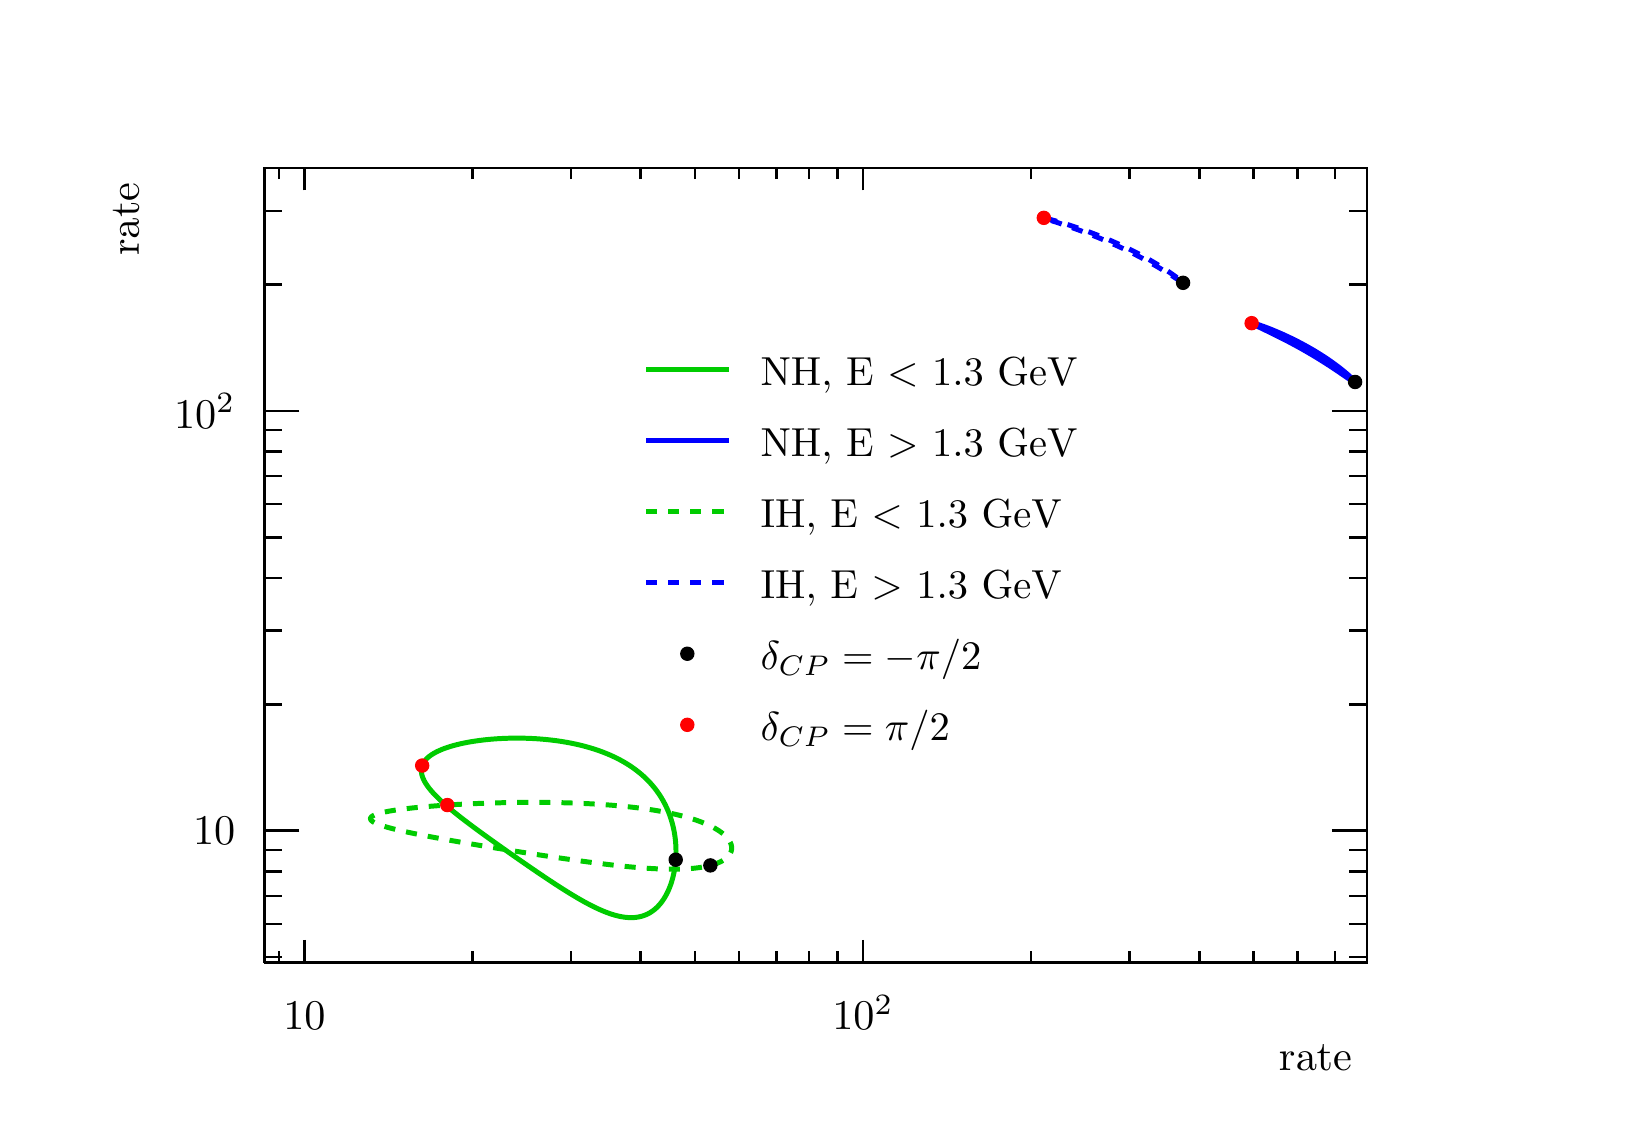
\begin{tikzpicture}
\pgfdeclareplotmark{cross} {
\pgfpathmoveto{\pgfpoint{-0.3\pgfplotmarksize}{\pgfplotmarksize}}
\pgfpathlineto{\pgfpoint{+0.3\pgfplotmarksize}{\pgfplotmarksize}}
\pgfpathlineto{\pgfpoint{+0.3\pgfplotmarksize}{0.3\pgfplotmarksize}}
\pgfpathlineto{\pgfpoint{+1\pgfplotmarksize}{0.3\pgfplotmarksize}}
\pgfpathlineto{\pgfpoint{+1\pgfplotmarksize}{-0.3\pgfplotmarksize}}
\pgfpathlineto{\pgfpoint{+0.3\pgfplotmarksize}{-0.3\pgfplotmarksize}}
\pgfpathlineto{\pgfpoint{+0.3\pgfplotmarksize}{-1.\pgfplotmarksize}}
\pgfpathlineto{\pgfpoint{-0.3\pgfplotmarksize}{-1.\pgfplotmarksize}}
\pgfpathlineto{\pgfpoint{-0.3\pgfplotmarksize}{-0.3\pgfplotmarksize}}
\pgfpathlineto{\pgfpoint{-1.\pgfplotmarksize}{-0.3\pgfplotmarksize}}
\pgfpathlineto{\pgfpoint{-1.\pgfplotmarksize}{0.3\pgfplotmarksize}}
\pgfpathlineto{\pgfpoint{-0.3\pgfplotmarksize}{0.3\pgfplotmarksize}}
\pgfpathclose
\pgfusepathqstroke
}
\pgfdeclareplotmark{cross*} {
\pgfpathmoveto{\pgfpoint{-0.3\pgfplotmarksize}{\pgfplotmarksize}}
\pgfpathlineto{\pgfpoint{+0.3\pgfplotmarksize}{\pgfplotmarksize}}
\pgfpathlineto{\pgfpoint{+0.3\pgfplotmarksize}{0.3\pgfplotmarksize}}
\pgfpathlineto{\pgfpoint{+1\pgfplotmarksize}{0.3\pgfplotmarksize}}
\pgfpathlineto{\pgfpoint{+1\pgfplotmarksize}{-0.3\pgfplotmarksize}}
\pgfpathlineto{\pgfpoint{+0.3\pgfplotmarksize}{-0.3\pgfplotmarksize}}
\pgfpathlineto{\pgfpoint{+0.3\pgfplotmarksize}{-1.\pgfplotmarksize}}
\pgfpathlineto{\pgfpoint{-0.3\pgfplotmarksize}{-1.\pgfplotmarksize}}
\pgfpathlineto{\pgfpoint{-0.3\pgfplotmarksize}{-0.3\pgfplotmarksize}}
\pgfpathlineto{\pgfpoint{-1.\pgfplotmarksize}{-0.3\pgfplotmarksize}}
\pgfpathlineto{\pgfpoint{-1.\pgfplotmarksize}{0.3\pgfplotmarksize}}
\pgfpathlineto{\pgfpoint{-0.3\pgfplotmarksize}{0.3\pgfplotmarksize}}
\pgfpathclose
\pgfusepathqfillstroke
}
\pgfdeclareplotmark{newstar} {
\pgfpathmoveto{\pgfqpoint{0pt}{\pgfplotmarksize}}
\pgfpathlineto{\pgfqpointpolar{44}{0.5\pgfplotmarksize}}
\pgfpathlineto{\pgfqpointpolar{18}{\pgfplotmarksize}}
\pgfpathlineto{\pgfqpointpolar{-20}{0.5\pgfplotmarksize}}
\pgfpathlineto{\pgfqpointpolar{-54}{\pgfplotmarksize}}
\pgfpathlineto{\pgfqpointpolar{-90}{0.5\pgfplotmarksize}}
\pgfpathlineto{\pgfqpointpolar{234}{\pgfplotmarksize}}
\pgfpathlineto{\pgfqpointpolar{198}{0.5\pgfplotmarksize}}
\pgfpathlineto{\pgfqpointpolar{162}{\pgfplotmarksize}}
\pgfpathlineto{\pgfqpointpolar{134}{0.5\pgfplotmarksize}}
\pgfpathclose
\pgfusepathqstroke
}
\pgfdeclareplotmark{newstar*} {
\pgfpathmoveto{\pgfqpoint{0pt}{\pgfplotmarksize}}
\pgfpathlineto{\pgfqpointpolar{44}{0.5\pgfplotmarksize}}
\pgfpathlineto{\pgfqpointpolar{18}{\pgfplotmarksize}}
\pgfpathlineto{\pgfqpointpolar{-20}{0.5\pgfplotmarksize}}
\pgfpathlineto{\pgfqpointpolar{-54}{\pgfplotmarksize}}
\pgfpathlineto{\pgfqpointpolar{-90}{0.5\pgfplotmarksize}}
\pgfpathlineto{\pgfqpointpolar{234}{\pgfplotmarksize}}
\pgfpathlineto{\pgfqpointpolar{198}{0.5\pgfplotmarksize}}
\pgfpathlineto{\pgfqpointpolar{162}{\pgfplotmarksize}}
\pgfpathlineto{\pgfqpointpolar{134}{0.5\pgfplotmarksize}}
\pgfpathclose
\pgfusepathqfillstroke
}
\definecolor{c}{rgb}{1,1,1};
\draw [color=c, fill=c] (0,0) rectangle (20,13.639);
\draw [color=c, fill=c] (3,1.77307) rectangle (17,11.8659);
\definecolor{c}{rgb}{0,0,0};
\draw [c,line width=0.9] (3,1.77307) -- (3,11.8659) -- (17,11.8659) -- (17,1.77307) -- (3,1.77307);
\definecolor{c}{rgb}{1,1,1};
\draw [color=c, fill=c] (3,1.77307) rectangle (17,11.8659);
\definecolor{c}{rgb}{0,0,0};
\draw [c,line width=0.9] (3,1.77307) -- (3,11.8659) -- (17,11.8659) -- (17,1.77307) -- (3,1.77307);
\draw [c,line width=0.9] (3,1.77307) -- (17,1.77307);
\draw [c,line width=0.9] (3.18294,1.91628) -- (3.18294,1.77307);
\draw [c,line width=0.9] (3.50753,2.05948) -- (3.50753,1.77307);
\draw [anchor=base] (3.50753,0.92063) node[scale=1.52731, color=c, rotate=0]{10};
\draw [c,line width=0.9] (5.64294,1.91628) -- (5.64294,1.77307);
\draw [c,line width=0.9] (6.89208,1.91628) -- (6.89208,1.77307);
\draw [c,line width=0.9] (7.77836,1.91628) -- (7.77836,1.77307);
\draw [c,line width=0.9] (8.46581,1.91628) -- (8.46581,1.77307);
\draw [c,line width=0.9] (9.0275,1.91628) -- (9.0275,1.77307);
\draw [c,line width=0.9] (9.5024,1.91628) -- (9.5024,1.77307);
\draw [c,line width=0.9] (9.91377,1.91628) -- (9.91377,1.77307);
\draw [c,line width=0.9] (10.2766,1.91628) -- (10.2766,1.77307);
\draw [c,line width=0.9] (10.6012,2.05948) -- (10.6012,1.77307);
\draw [anchor=base] (10.6012,0.92063) node[scale=1.52731, color=c, rotate=0]{$10^{2}$};
\draw [c,line width=0.9] (12.7366,1.91628) -- (12.7366,1.77307);
\draw [c,line width=0.9] (13.9858,1.91628) -- (13.9858,1.77307);
\draw [c,line width=0.9] (14.8721,1.91628) -- (14.8721,1.77307);
\draw [c,line width=0.9] (15.5595,1.91628) -- (15.5595,1.77307);
\draw [c,line width=0.9] (16.1212,1.91628) -- (16.1212,1.77307);
\draw [c,line width=0.9] (16.5961,1.91628) -- (16.5961,1.77307);
\draw [anchor= east] (17,0.572837) node[scale=1.52731, color=c, rotate=0]{\nue rate};
\draw [c,line width=0.9] (3,11.8659) -- (17,11.8659);
\draw [c,line width=0.9] (3.18294,11.7227) -- (3.18294,11.8659);
\draw [c,line width=0.9] (3.50753,11.5795) -- (3.50753,11.8659);
\draw [c,line width=0.9] (5.64294,11.7227) -- (5.64294,11.8659);
\draw [c,line width=0.9] (6.89208,11.7227) -- (6.89208,11.8659);
\draw [c,line width=0.9] (7.77836,11.7227) -- (7.77836,11.8659);
\draw [c,line width=0.9] (8.46581,11.7227) -- (8.46581,11.8659);
\draw [c,line width=0.9] (9.0275,11.7227) -- (9.0275,11.8659);
\draw [c,line width=0.9] (9.5024,11.7227) -- (9.5024,11.8659);
\draw [c,line width=0.9] (9.91377,11.7227) -- (9.91377,11.8659);
\draw [c,line width=0.9] (10.2766,11.7227) -- (10.2766,11.8659);
\draw [c,line width=0.9] (10.6012,11.5795) -- (10.6012,11.8659);
\draw [c,line width=0.9] (12.7366,11.7227) -- (12.7366,11.8659);
\draw [c,line width=0.9] (13.9858,11.7227) -- (13.9858,11.8659);
\draw [c,line width=0.9] (14.8721,11.7227) -- (14.8721,11.8659);
\draw [c,line width=0.9] (15.5595,11.7227) -- (15.5595,11.8659);
\draw [c,line width=0.9] (16.1212,11.7227) -- (16.1212,11.8659);
\draw [c,line width=0.9] (16.5961,11.7227) -- (16.5961,11.8659);
\draw [c,line width=0.9] (3,1.77307) -- (3,11.8659);
\draw [c,line width=0.9] (3.222,1.84242) -- (3,1.84242);
\draw [c,line width=0.9] (3.222,2.26449) -- (3,2.26449);
\draw [c,line width=0.9] (3.222,2.62135) -- (3,2.62135);
\draw [c,line width=0.9] (3.222,2.93047) -- (3,2.93047);
\draw [c,line width=0.9] (3.222,3.20314) -- (3,3.20314);
\draw [c,line width=0.9] (3.444,3.44704) -- (3,3.44704);
\draw [anchor= east] (2.82,3.44704) node[scale=1.52731, color=c, rotate=0]{10};
\draw [c,line width=0.9] (3.222,5.05166) -- (3,5.05166);
\draw [c,line width=0.9] (3.222,5.9903) -- (3,5.9903);
\draw [c,line width=0.9] (3.222,6.65628) -- (3,6.65628);
\draw [c,line width=0.9] (3.222,7.17285) -- (3,7.17285);
\draw [c,line width=0.9] (3.222,7.59492) -- (3,7.59492);
\draw [c,line width=0.9] (3.222,7.95178) -- (3,7.95178);
\draw [c,line width=0.9] (3.222,8.2609) -- (3,8.2609);
\draw [c,line width=0.9] (3.222,8.53357) -- (3,8.53357);
\draw [c,line width=0.9] (3.444,8.77747) -- (3,8.77747);
\draw [anchor= east] (2.82,8.77747) node[scale=1.52731, color=c, rotate=0]{$10^{2}$};
\draw [c,line width=0.9] (3.222,10.3821) -- (3,10.3821);
\draw [c,line width=0.9] (3.222,11.3207) -- (3,11.3207);
\draw [anchor= east] (1.24,11.8659) node[scale=1.52731, color=c, rotate=90]{\anue rate};
\draw [c,line width=0.9] (17,1.77307) -- (17,11.8659);
\draw [c,line width=0.9] (16.778,1.84242) -- (17,1.84242);
\draw [c,line width=0.9] (16.778,2.26449) -- (17,2.26449);
\draw [c,line width=0.9] (16.778,2.62135) -- (17,2.62135);
\draw [c,line width=0.9] (16.778,2.93047) -- (17,2.93047);
\draw [c,line width=0.9] (16.778,3.20314) -- (17,3.20314);
\draw [c,line width=0.9] (16.556,3.44704) -- (17,3.44704);
\draw [c,line width=0.9] (16.778,5.05166) -- (17,5.05166);
\draw [c,line width=0.9] (16.778,5.9903) -- (17,5.9903);
\draw [c,line width=0.9] (16.778,6.65628) -- (17,6.65628);
\draw [c,line width=0.9] (16.778,7.17285) -- (17,7.17285);
\draw [c,line width=0.9] (16.778,7.59492) -- (17,7.59492);
\draw [c,line width=0.9] (16.778,7.95178) -- (17,7.95178);
\draw [c,line width=0.9] (16.778,8.2609) -- (17,8.2609);
\draw [c,line width=0.9] (16.778,8.53357) -- (17,8.53357);
\draw [c,line width=0.9] (16.556,8.77747) -- (17,8.77747);
\draw [c,line width=0.9] (16.778,10.3821) -- (17,10.3821);
\draw [c,line width=0.9] (16.778,11.3207) -- (17,11.3207);
\definecolor{c}{rgb}{0,0.8,0};
\draw [c,line width=1.8] (6.88511,2.64748) -- (6.93323,2.61837) -- (6.98069,2.59036) -- (7.02747,2.56352) -- (7.07353,2.53791) -- (7.11886,2.51361) -- (7.16343,2.49069) -- (7.20723,2.46921) -- (7.25024,2.44924) -- (7.29243,2.43084) --
 (7.33379,2.41407) -- (7.37432,2.39898) -- (7.41398,2.38561) -- (7.45278,2.37402) -- (7.4907,2.36424) -- (7.52773,2.3563) -- (7.56386,2.35024) -- (7.59908,2.34606) -- (7.63339,2.34379) -- (7.66677,2.34344) -- (7.69922,2.345) -- (7.73073,2.34848) --
 (7.7613,2.35385) -- (7.79092,2.3611) -- (7.81959,2.3702) -- (7.84731,2.38113) -- (7.87406,2.39385) -- (7.89986,2.40831) -- (7.92468,2.42447) -- (7.94854,2.44228) -- (7.97142,2.46167) -- (7.99333,2.4826) -- (8.01427,2.505) -- (8.03423,2.5288) --
 (8.05321,2.55393) -- (8.07121,2.58032) -- (8.08822,2.60791) -- (8.10426,2.63662) -- (8.11931,2.66638) -- (8.13338,2.69711) -- (8.14646,2.72874) -- (8.15856,2.7612) -- (8.16967,2.79441) -- (8.1798,2.82832) -- (8.18894,2.86283) -- (8.19709,2.8979) --
 (8.20425,2.93345) -- (8.21043,2.96942) -- (8.21562,3.00574) -- (8.21982,3.04236) -- (8.22303,3.07922) -- (8.22526,3.11626) -- (8.22649,3.15343) -- (8.22674,3.19068) -- (8.226,3.22796) -- (8.22428,3.26522) -- (8.22156,3.30241) -- (8.21786,3.3395) --
 (8.21317,3.37645) -- (8.20749,3.41322) -- (8.20082,3.44976) -- (8.19316,3.48605) -- (8.18452,3.52206) -- (8.17489,3.55776) -- (8.16428,3.5931) -- (8.15268,3.62808) -- (8.14009,3.66267) -- (8.12652,3.69683) -- (8.11196,3.73055) -- (8.09642,3.76382)
 -- (8.0799,3.7966) -- (8.06239,3.82888) -- (8.0439,3.86064) -- (8.02444,3.89187) -- (8.00399,3.92256) -- (7.98257,3.95268) -- (7.96018,3.98224) -- (7.93681,4.0112) -- (7.91247,4.03957) -- (7.88717,4.06734) -- (7.8609,4.09449) -- (7.83366,4.12102) --
 (7.80547,4.14691) -- (7.77633,4.17216) -- (7.74624,4.19677) -- (7.7152,4.22073) -- (7.68322,4.24402) -- (7.6503,4.26665) -- (7.61646,4.28861) -- (7.5817,4.3099) -- (7.54603,4.33051) -- (7.50945,4.35044) -- (7.47198,4.36969) -- (7.43362,4.38824) --
 (7.39439,4.40611) -- (7.3543,4.42328) -- (7.31336,4.43975) -- (7.27158,4.45553) -- (7.22898,4.4706) -- (7.18558,4.48498) -- (7.14139,4.49865) -- (7.09644,4.51161) -- (7.05074,4.52387) -- (7.00432,4.53542) -- (6.9572,4.54625) -- (6.90941,4.55638) --
 (6.86098,4.5658) -- (6.81193,4.57451) -- (6.76229,4.5825) -- (6.71211,4.58978) -- (6.66142,4.59635) -- (6.61026,4.60221) -- (6.55867,4.60735) -- (6.5067,4.61177) -- (6.45439,4.61548) -- (6.40179,4.61847) -- (6.34897,4.62075) -- (6.29596,4.62232) --
 (6.24285,4.62316) -- (6.18969,4.6233) -- (6.13654,4.62271) -- (6.08349,4.62141) -- (6.03059,4.6194) -- (5.97794,4.61667) -- (5.92562,4.61322) -- (5.8737,4.60906) -- (5.82228,4.60418) -- (5.77145,4.59859) -- (5.7213,4.59229) -- (5.67194,4.58527) --
 (5.62347,4.57754) -- (5.57599,4.5691) -- (5.5296,4.55994) -- (5.48442,4.55007) -- (5.44055,4.53949) -- (5.3981,4.52821) -- (5.35719,4.51621) -- (5.31793,4.50351) -- (5.28043,4.4901) -- (5.24479,4.47599) -- (5.21112,4.46117) -- (5.17953,4.44565) --
 (5.15011,4.42943) -- (5.12296,4.41252) -- (5.09818,4.39491) -- (5.07584,4.37661) -- (5.05602,4.35762) -- (5.03879,4.33794) -- (5.02422,4.31758) -- (5.01235,4.29654) -- (5.00323,4.27483) -- (4.99689,4.25244) -- (4.99336,4.22939) -- (4.99265,4.20568)
 -- (4.99476,4.18131) -- (4.99969,4.15629) -- (5.00741,4.13064) -- (5.0179,4.10434) -- (5.03112,4.07742) -- (5.04702,4.04988) -- (5.06554,4.02173) -- (5.08662,3.99298) -- (5.11019,3.96365) -- (5.13615,3.93373) -- (5.16444,3.90325) --
 (5.19495,3.87222) -- (5.22758,3.84065) -- (5.26225,3.80856) -- (5.29882,3.77596) -- (5.33722,3.74287) -- (5.37731,3.70932) -- (5.419,3.67531) -- (5.46216,3.64088) -- (5.5067,3.60605) -- (5.55249,3.57083) -- (5.59944,3.53526) -- (5.64743,3.49937) --
 (5.69635,3.46317) -- (5.74611,3.42672) -- (5.79661,3.39003) -- (5.84775,3.35315) -- (5.89943,3.3161) -- (5.95156,3.27894) -- (6.00406,3.2417) -- (6.05684,3.20442) -- (6.10982,3.16716) -- (6.16293,3.12995) -- (6.21609,3.09286) -- (6.26924,3.05593) --
 (6.3223,3.01921) -- (6.37523,2.98277) -- (6.42794,2.94666) -- (6.4804,2.91095) -- (6.53255,2.8757) -- (6.58434,2.84097) -- (6.63573,2.80684) -- (6.68666,2.77336) -- (6.7371,2.74061) -- (6.78701,2.70867) -- (6.83636,2.6776) -- (6.88511,2.64748);
\definecolor{c}{rgb}{0,0,1};
\draw [c,line width=1.8] (16.305,9.49028) -- (16.325,9.47835) -- (16.3448,9.46643) -- (16.3644,9.45453) -- (16.3837,9.44267) -- (16.4028,9.43085) -- (16.4217,9.4191) -- (16.4403,9.40742) -- (16.4586,9.39582) -- (16.4767,9.38432) -- (16.4944,9.37294)
 -- (16.5118,9.36168) -- (16.5289,9.35056) -- (16.5456,9.33959) -- (16.562,9.32879) -- (16.578,9.31817) -- (16.5936,9.30774) -- (16.6089,9.29752) -- (16.6237,9.28751) -- (16.6382,9.27774) -- (16.6522,9.26821) -- (16.6658,9.25893) -- (16.679,9.24993)
 -- (16.6917,9.24121) -- (16.704,9.23278) -- (16.7159,9.22466) -- (16.7273,9.21686) -- (16.7382,9.20938) -- (16.7486,9.20224) -- (16.7586,9.19545) -- (16.7681,9.18902) -- (16.7771,9.18296) -- (16.7856,9.17728) -- (16.7936,9.17198) --
 (16.8011,9.16707) -- (16.8081,9.16257) -- (16.8146,9.15847) -- (16.8206,9.15479) -- (16.8261,9.15152) -- (16.8311,9.14869) -- (16.8355,9.14628) -- (16.8395,9.1443) -- (16.8429,9.14276) -- (16.8457,9.14165) -- (16.8481,9.14099) -- (16.8499,9.14077)
 -- (16.8512,9.14099) -- (16.852,9.14165) -- (16.8522,9.14275) -- (16.8519,9.14429) -- (16.8511,9.14626) -- (16.8498,9.14867) -- (16.8479,9.1515) -- (16.8455,9.15477) -- (16.8426,9.15845) -- (16.8391,9.16254) -- (16.8352,9.16704) -- (16.8307,9.17194)
 -- (16.8257,9.17724) -- (16.8201,9.18292) -- (16.8141,9.18898) -- (16.8075,9.19541) -- (16.8005,9.2022) -- (16.7929,9.20933) -- (16.7849,9.21681) -- (16.7763,9.22461) -- (16.7673,9.23273) -- (16.7577,9.24116) -- (16.7477,9.24988) --
 (16.7372,9.25888) -- (16.7262,9.26815) -- (16.7148,9.27767) -- (16.7029,9.28745) -- (16.6906,9.29745) -- (16.6778,9.30767) -- (16.6646,9.3181) -- (16.651,9.32872) -- (16.6369,9.33952) -- (16.6224,9.35049) -- (16.6075,9.36161) -- (16.5922,9.37286) --
 (16.5766,9.38425) -- (16.5605,9.39575) -- (16.5441,9.40734) -- (16.5274,9.41902) -- (16.5102,9.43078) -- (16.4928,9.44259) -- (16.4751,9.45446) -- (16.457,9.46636) -- (16.4387,9.47828) -- (16.42,9.49021) -- (16.4011,9.50214) -- (16.382,9.51405) --
 (16.3626,9.52594) -- (16.343,9.53779) -- (16.3232,9.54959) -- (16.3032,9.56134) -- (16.2831,9.57301) -- (16.2627,9.5846) -- (16.2423,9.5961) -- (16.2217,9.60749) -- (16.2011,9.61878) -- (16.1803,9.62994) -- (16.1596,9.64097) -- (16.1387,9.65187) --
 (16.1179,9.66261) -- (16.0971,9.67319) -- (16.0763,9.68361) -- (16.0555,9.69386) -- (16.0348,9.70392) -- (16.0142,9.71379) -- (15.9938,9.72346) -- (15.9734,9.73293) -- (15.9533,9.74219) -- (15.9333,9.75122) -- (15.9136,9.76004) -- (15.8941,9.76862)
 -- (15.8748,9.77697) -- (15.8559,9.78507) -- (15.8372,9.79292) -- (15.8189,9.80052) -- (15.801,9.80786) -- (15.7835,9.81494) -- (15.7664,9.82175) -- (15.7497,9.82829) -- (15.7335,9.83455) -- (15.7177,9.84052) -- (15.7025,9.84622) --
 (15.6878,9.85163) -- (15.6737,9.85674) -- (15.6601,9.86156) -- (15.6472,9.86609) -- (15.6349,9.87031) -- (15.6232,9.87423) -- (15.6122,9.87784) -- (15.6018,9.88115) -- (15.5922,9.88415) -- (15.5832,9.88684) -- (15.575,9.88922) -- (15.5676,9.89128)
 -- (15.5609,9.89302) -- (15.5549,9.89446) -- (15.5497,9.89557) -- (15.5454,9.89637) -- (15.5418,9.89684) -- (15.539,9.89701) -- (15.537,9.89685) -- (15.5358,9.89637) -- (15.5354,9.89558) -- (15.5359,9.89446) -- (15.5371,9.89303) -- (15.5392,9.89129)
 -- (15.5421,9.88923) -- (15.5457,9.88686) -- (15.5502,9.88417) -- (15.5554,9.88117) -- (15.5614,9.87787) -- (15.5682,9.87425) -- (15.5757,9.87033) -- (15.584,9.86611) -- (15.593,9.86159) -- (15.6027,9.85677) -- (15.6131,9.85166) -- (15.6242,9.84626)
 -- (15.636,9.84056) -- (15.6483,9.83459) -- (15.6613,9.82833) -- (15.6749,9.82179) -- (15.6891,9.81498) -- (15.7039,9.80791) -- (15.7191,9.80057) -- (15.7349,9.79297) -- (15.7512,9.78512) -- (15.7679,9.77702) -- (15.785,9.76867) -- (15.8026,9.76009)
 -- (15.8206,9.75128) -- (15.8389,9.74225) -- (15.8576,9.73299) -- (15.8765,9.72352) -- (15.8958,9.71385) -- (15.9153,9.70398) -- (15.9351,9.69392) -- (15.9551,9.68368) -- (15.9753,9.67326) -- (15.9956,9.66268) -- (16.0161,9.65194) --
 (16.0367,9.64105) -- (16.0574,9.63001) -- (16.0781,9.61885) -- (16.0989,9.60757) -- (16.1198,9.59617) -- (16.1406,9.58467) -- (16.1614,9.57308) -- (16.1822,9.56141) -- (16.2029,9.54967) -- (16.2236,9.53787) -- (16.2441,9.52602) -- (16.2646,9.51413)
 -- (16.2849,9.50221) -- (16.305,9.49028);
\definecolor{c}{rgb}{0,0.8,0};
\draw [c,dash pattern=on 4.00pt off 4.00pt ,line width=1.8] (8.44666,3.59344) -- (8.4804,3.58226) -- (8.51291,3.57086) -- (8.54417,3.55927) -- (8.57421,3.54748) -- (8.60302,3.53552) -- (8.63061,3.52338) -- (8.65697,3.51108) -- (8.68212,3.49862) --
 (8.70605,3.48602) -- (8.72877,3.47329) -- (8.75028,3.46044) -- (8.77059,3.44748) -- (8.7897,3.43442) -- (8.80761,3.42128) -- (8.82432,3.40805) -- (8.83983,3.39477) -- (8.85416,3.38144) -- (8.86729,3.36807) -- (8.87924,3.35467) -- (8.89,3.34127) --
 (8.89957,3.32787) -- (8.90797,3.31448) -- (8.91518,3.30113) -- (8.92121,3.28782) -- (8.92606,3.27457) -- (8.92974,3.26139) -- (8.93223,3.24831) -- (8.93355,3.23533) -- (8.93369,3.22247) -- (8.93266,3.20974) -- (8.93044,3.19716) -- (8.92705,3.18475)
 -- (8.92248,3.17252) -- (8.91673,3.16048) -- (8.9098,3.14865) -- (8.90169,3.13706) -- (8.8924,3.1257) -- (8.88192,3.1146) -- (8.87025,3.10377) -- (8.8574,3.09323) -- (8.84336,3.08299) -- (8.82813,3.07307) -- (8.81171,3.06348) -- (8.79409,3.05423) --
 (8.77527,3.04533) -- (8.75525,3.03681) -- (8.73402,3.02867) -- (8.71159,3.02093) -- (8.68795,3.01359) -- (8.66309,3.00668) -- (8.63702,3.00019) -- (8.60973,2.99414) -- (8.58121,2.98854) -- (8.55147,2.98339) -- (8.52049,2.97871) -- (8.48829,2.97451)
 -- (8.45484,2.97078) -- (8.42016,2.96755) -- (8.38423,2.9648) -- (8.34705,2.96254) -- (8.30863,2.96079) -- (8.26895,2.95954) -- (8.22801,2.95879) -- (8.18582,2.95855) -- (8.14236,2.95882) -- (8.09764,2.95959) -- (8.05166,2.96086) --
 (8.00442,2.96264) -- (7.95591,2.96491) -- (7.90613,2.96768) -- (7.85509,2.97094) -- (7.80278,2.97469) -- (7.74922,2.97892) -- (7.6944,2.98362) -- (7.63833,2.98878) -- (7.58101,2.9944) -- (7.52245,3.00047) -- (7.46265,3.00698) -- (7.40164,3.01392) --
 (7.33942,3.02127) -- (7.276,3.02903) -- (7.21141,3.03719) -- (7.14565,3.04573) -- (7.07876,3.05464) -- (7.01075,3.0639) -- (6.94165,3.07351) -- (6.87149,3.08345) -- (6.80031,3.0937) -- (6.72815,3.10426) -- (6.65505,3.1151) -- (6.58105,3.12621) --
 (6.50622,3.13758) -- (6.43061,3.14919) -- (6.35428,3.16102) -- (6.2773,3.17307) -- (6.19977,3.18531) -- (6.12175,3.19773) -- (6.04335,3.21031) -- (5.96467,3.22305) -- (5.88581,3.23591) -- (5.80691,3.2489) -- (5.72809,3.26199) -- (5.64949,3.27517) --
 (5.57127,3.28842) -- (5.49358,3.30173) -- (5.4166,3.31509) -- (5.34051,3.32847) -- (5.26552,3.34188) -- (5.19181,3.35528) -- (5.11961,3.36867) -- (5.04915,3.38204) -- (4.98065,3.39537) -- (4.91436,3.40865) -- (4.85052,3.42187) -- (4.78939,3.43501)
 -- (4.73121,3.44807) -- (4.67623,3.46103) -- (4.62472,3.47387) -- (4.57691,3.4866) -- (4.53304,3.49919) -- (4.49333,3.51164) -- (4.458,3.52393) -- (4.42723,3.53606) -- (4.40121,3.54802) -- (4.38007,3.5598) -- (4.36396,3.57138) -- (4.35294,3.58277)
 -- (4.34711,3.59394) -- (4.34649,3.6049) -- (4.35108,3.61564) -- (4.36086,3.62614) -- (4.37576,3.6364) -- (4.39571,3.64642) -- (4.42057,3.65618) -- (4.45022,3.66568) -- (4.48448,3.67492) -- (4.52316,3.68388) -- (4.56605,3.69257) -- (4.61294,3.70097)
 -- (4.66359,3.70908) -- (4.71776,3.7169) -- (4.7752,3.72441) -- (4.83565,3.73163) -- (4.89887,3.73853) -- (4.96459,3.74513) -- (5.03259,3.75141) -- (5.1026,3.75737) -- (5.17441,3.763) -- (5.24777,3.76831) -- (5.32248,3.77329) -- (5.39832,3.77794) --
 (5.4751,3.78225) -- (5.55264,3.78623) -- (5.63075,3.78987) -- (5.70927,3.79316) -- (5.78805,3.79612) -- (5.86695,3.79873) -- (5.94583,3.80099) -- (6.02456,3.8029) -- (6.10304,3.80447) -- (6.18115,3.80569) -- (6.25881,3.80656) -- (6.33593,3.80708) --
 (6.41242,3.80724) -- (6.48821,3.80706) -- (6.56324,3.80653) -- (6.63744,3.80564) -- (6.71076,3.80441) -- (6.78315,3.80283) -- (6.85457,3.80089) -- (6.92497,3.79862) -- (6.99432,3.79599) -- (7.0626,3.79302) -- (7.12976,3.78971) -- (7.19579,3.78606)
 -- (7.26067,3.78207) -- (7.32437,3.77774) -- (7.38688,3.77307) -- (7.44818,3.76808) -- (7.50826,3.76275) -- (7.56712,3.7571) -- (7.62474,3.75113) -- (7.68111,3.74484) -- (7.73623,3.73823) -- (7.79009,3.73131) -- (7.8427,3.72408) -- (7.89404,3.71655)
 -- (7.94412,3.70872) -- (7.99293,3.70059) -- (8.04048,3.69218) -- (8.08677,3.68348) -- (8.13179,3.67451) -- (8.17554,3.66526) -- (8.21804,3.65575) -- (8.25927,3.64597) -- (8.29925,3.63595) -- (8.33798,3.62567) -- (8.37545,3.61516) --
 (8.41168,3.60441) -- (8.44666,3.59344);
\definecolor{c}{rgb}{0,0,1};
\draw [c,dash pattern=on 4.00pt off 4.00pt ,line width=1.8] (13.9856,10.8326) -- (14.0118,10.8196) -- (14.0377,10.8066) -- (14.0632,10.7936) -- (14.0884,10.7805) -- (14.1132,10.7675) -- (14.1377,10.7544) -- (14.1617,10.7414) -- (14.1853,10.7285) --
 (14.2084,10.7156) -- (14.2311,10.7027) -- (14.2533,10.69) -- (14.2751,10.6773) -- (14.2963,10.6648) -- (14.3171,10.6524) -- (14.3373,10.6401) -- (14.357,10.628) -- (14.3762,10.616) -- (14.3948,10.6043) -- (14.4129,10.5927) -- (14.4304,10.5814) --
 (14.4474,10.5703) -- (14.4637,10.5594) -- (14.4795,10.5488) -- (14.4947,10.5385) -- (14.5093,10.5285) -- (14.5232,10.5188) -- (14.5366,10.5094) -- (14.5494,10.5003) -- (14.5615,10.4916) -- (14.573,10.4832) -- (14.5839,10.4752) -- (14.5941,10.4675)
 -- (14.6037,10.4603) -- (14.6127,10.4535) -- (14.621,10.447) -- (14.6286,10.4411) -- (14.6356,10.4355) -- (14.642,10.4304) -- (14.6477,10.4257) -- (14.6527,10.4215) -- (14.6571,10.4177) -- (14.6608,10.4144) -- (14.6638,10.4116) -- (14.6662,10.4093)
 -- (14.6679,10.4074) -- (14.669,10.4061) -- (14.6694,10.4052) -- (14.6691,10.4048) -- (14.6682,10.4049) -- (14.6666,10.4055) -- (14.6643,10.4066) -- (14.6613,10.4082) -- (14.6577,10.4102) -- (14.6535,10.4128) -- (14.6486,10.4158) -- (14.643,10.4193)
 -- (14.6367,10.4232) -- (14.6298,10.4276) -- (14.6223,10.4325) -- (14.6141,10.4378) -- (14.6052,10.4436) -- (14.5958,10.4497) -- (14.5856,10.4563) -- (14.5749,10.4633) -- (14.5635,10.4708) -- (14.5514,10.4785) -- (14.5388,10.4867) --
 (14.5255,10.4952) -- (14.5117,10.5041) -- (14.4972,10.5134) -- (14.4821,10.5229) -- (14.4664,10.5328) -- (14.4501,10.5429) -- (14.4333,10.5533) -- (14.4159,10.5641) -- (14.3979,10.575) -- (14.3794,10.5862) -- (14.3603,10.5976) -- (14.3406,10.6093)
 -- (14.3205,10.6211) -- (14.2998,10.6331) -- (14.2787,10.6453) -- (14.257,10.6577) -- (14.2348,10.6701) -- (14.2122,10.6827) -- (14.1892,10.6954) -- (14.1656,10.7082) -- (14.1417,10.7211) -- (14.1173,10.734) -- (14.0926,10.747) -- (14.0675,10.76) --
 (14.042,10.7731) -- (14.0162,10.7861) -- (13.99,10.7992) -- (13.9635,10.8122) -- (13.9368,10.8252) -- (13.9098,10.8381) -- (13.8825,10.851) -- (13.855,10.8639) -- (13.8274,10.8766) -- (13.7995,10.8893) -- (13.7716,10.9018) -- (13.7435,10.9143) --
 (13.7153,10.9266) -- (13.687,10.9388) -- (13.6588,10.9508) -- (13.6305,10.9627) -- (13.6022,10.9744) -- (13.574,10.986) -- (13.5459,10.9973) -- (13.5179,11.0085) -- (13.4901,11.0195) -- (13.4624,11.0302) -- (13.435,11.0408) -- (13.4078,11.0511) --
 (13.381,11.0612) -- (13.3545,11.071) -- (13.3283,11.0807) -- (13.3026,11.09) -- (13.2773,11.0991) -- (13.2525,11.108) -- (13.2282,11.1165) -- (13.2045,11.1248) -- (13.1814,11.1328) -- (13.1589,11.1406) -- (13.1371,11.148) -- (13.1161,11.1552) --
 (13.0957,11.162) -- (13.0762,11.1685) -- (13.0575,11.1748) -- (13.0396,11.1807) -- (13.0226,11.1863) -- (13.0066,11.1916) -- (12.9915,11.1966) -- (12.9774,11.2012) -- (12.9643,11.2055) -- (12.9522,11.2095) -- (12.9412,11.2132) -- (12.9313,11.2165)
 -- (12.9225,11.2195) -- (12.9148,11.2222) -- (12.9083,11.2245) -- (12.9029,11.2264) -- (12.8986,11.2281) -- (12.8956,11.2294) -- (12.8937,11.2303) -- (12.893,11.231) -- (12.8935,11.2312) -- (12.8952,11.2311) -- (12.898,11.2307) -- (12.9021,11.23) --
 (12.9073,11.2289) -- (12.9136,11.2274) -- (12.9211,11.2256) -- (12.9297,11.2235) -- (12.9395,11.2211) -- (12.9503,11.2183) -- (12.9622,11.2151) -- (12.9751,11.2117) -- (12.9891,11.2079) -- (13.004,11.2037) -- (13.0199,11.1993) -- (13.0367,11.1945)
 -- (13.0544,11.1894) -- (13.073,11.1839) -- (13.0924,11.1782) -- (13.1126,11.1721) -- (13.1336,11.1658) -- (13.1552,11.1591) -- (13.1776,11.1521) -- (13.2006,11.1449) -- (13.2242,11.1373) -- (13.2484,11.1294) -- (13.2731,11.1213) --
 (13.2983,11.1129) -- (13.324,11.1042) -- (13.3501,11.0953) -- (13.3765,11.086) -- (13.4033,11.0766) -- (13.4304,11.0669) -- (13.4578,11.0569) -- (13.4854,11.0467) -- (13.5132,11.0363) -- (13.5412,11.0256) -- (13.5693,11.0148) -- (13.5975,11.0037) --
 (13.6257,10.9925) -- (13.654,10.981) -- (13.6823,10.9694) -- (13.7106,10.9576) -- (13.7388,10.9457) -- (13.7669,10.9336) -- (13.7949,10.9213) -- (13.8227,10.909) -- (13.8504,10.8965) -- (13.8779,10.8839) -- (13.9052,10.8712) -- (13.9323,10.8584) --
 (13.9591,10.8455) -- (13.9856,10.8326);
\definecolor{c}{rgb}{1,1,1};
\draw [color=c, fill=c] (2,12.8206) rectangle (18,13.5708);
\definecolor{c}{rgb}{0,0,0};
%\draw (10,13.1957) node[scale=1.40004, color=c, rotate=0]{$Comparison of \nu_{e} rates at the DUNE far detector$};
\foreach \P in {(8.22303,3.07922)}{\draw[mark options={color=c,fill=c},mark size=2.402402pt,mark=*] plot coordinates {\P};}
\definecolor{c}{rgb}{1,0,0};
\foreach \P in {(5.00323,4.27483)}{\draw[mark options={color=c,fill=c},mark size=2.402402pt,mark=*] plot coordinates {\P};}
\foreach \P in {(5.32248,3.77329)}{\draw[mark options={color=c,fill=c},mark size=2.402402pt,mark=*] plot coordinates {\P};}
\definecolor{c}{rgb}{0,0,0};
\foreach \P in {(8.66309,3.00668)}{\draw[mark options={color=c,fill=c},mark size=2.402402pt,mark=*] plot coordinates {\P};}
\foreach \P in {(14.6666,10.4055)}{\draw[mark options={color=c,fill=c},mark size=2.402402pt,mark=*] plot coordinates {\P};}
\definecolor{c}{rgb}{1,0,0};
\foreach \P in {(12.898,11.2307)}{\draw[mark options={color=c,fill=c},mark size=2.402402pt,mark=*] plot coordinates {\P};}
\foreach \P in {(15.5371,9.89303)}{\draw[mark options={color=c,fill=c},mark size=2.402402pt,mark=*] plot coordinates {\P};}
\definecolor{c}{rgb}{0,0,0};
\foreach \P in {(16.8511,9.14626)}{\draw[mark options={color=c,fill=c},mark size=2.402402pt,mark=*] plot coordinates {\P};}
\definecolor{c}{rgb}{1,1,1};
\draw [color=c, fill=c] (7.62178,4.34097) rectangle (13.6103,9.75645);
\definecolor{c}{rgb}{0,0,0};
\draw [anchor=base west] (9.11891,9.10208) node[scale=1.46368, color=c, rotate=0]{NH, E $<$ 1.3 GeV};
\definecolor{c}{rgb}{1,1,1};
\draw [c, fill=c] (7.84635,8.98925) -- (8.89434,8.98925) -- (8.89434,9.62106) -- (7.84635,9.62106);
\definecolor{c}{rgb}{0,0.8,0};
\draw [c,line width=1.8] (7.84635,9.30516) -- (8.89434,9.30516);
\definecolor{c}{rgb}{0,0,0};
\draw [anchor=base west] (9.11891,8.1995) node[scale=1.46368, color=c, rotate=0]{NH, E $>$ 1.3 GeV};
\definecolor{c}{rgb}{1,1,1};
\draw [c, fill=c] (7.84635,8.08668) -- (8.89434,8.08668) -- (8.89434,8.71848) -- (7.84635,8.71848);
\definecolor{c}{rgb}{0,0,1};
\draw [c,line width=1.8] (7.84635,8.40258) -- (8.89434,8.40258);
\definecolor{c}{rgb}{0,0,0};
\draw [anchor=base west] (9.11891,7.29692) node[scale=1.46368, color=c, rotate=0]{IH, E $<$ 1.3 GeV};
\definecolor{c}{rgb}{1,1,1};
\draw [c, fill=c] (7.84635,7.1841) -- (8.89434,7.1841) -- (8.89434,7.8159) -- (7.84635,7.8159);
\definecolor{c}{rgb}{0,0.8,0};
\draw [c,dash pattern=on 4.00pt off 4.00pt ,line width=1.8] (7.84635,7.5) -- (8.89434,7.5);
\definecolor{c}{rgb}{0,0,0};
\draw [anchor=base west] (9.11891,6.39434) node[scale=1.46368, color=c, rotate=0]{IH, E $>$ 1.3 GeV};
\definecolor{c}{rgb}{1,1,1};
\draw [c, fill=c] (7.84635,6.28152) -- (8.89434,6.28152) -- (8.89434,6.91332) -- (7.84635,6.91332);
\definecolor{c}{rgb}{0,0,1};
\draw [c,dash pattern=on 4.00pt off 4.00pt ,line width=1.8] (7.84635,6.59742) -- (8.89434,6.59742);
\definecolor{c}{rgb}{0,0,0};
\draw [anchor=base west] (9.11891,5.49176) node[scale=1.46368, color=c, rotate=0]{$\delta_{CP}=-\pi/2$};
\foreach \P in {(8.37034,5.69484)}{\draw[mark options={color=c,fill=c},mark size=2.402402pt,mark=*] plot coordinates {\P};}
\draw [anchor=base west] (9.11891,4.58918) node[scale=1.46368, color=c, rotate=0]{$\delta_{CP}=\pi/2$};
\definecolor{c}{rgb}{1,0,0};
\foreach \P in {(8.37034,4.79226)}{\draw[mark options={color=c,fill=c},mark size=2.402402pt,mark=*] plot coordinates {\P};}
\end{tikzpicture}

    \end{adjustbox}
  \end{minipage}
  \caption[Predicted \nue and \anue rates for different values of \dcp and neutrino mass hierarchies at the first and second oscillation maxima.]{Comparison of predicted \nue and \anue rates in the DUNE far detector at the first (blue) and second (green) oscillation maxima and for normal (solid) and inverted (dashed) neutrino mass hierarchies. The right plot shows the same information but with logarithmic axes.}
  \label{fig:nueRates}
\end{figure}

One can see in the right-hand plot of \citefig{fig:nueRates} that there is considerable overlap between the ellipses traced by the rates at the second oscillation maximum.
In particular, the maximally CP-violating points ($\dcp=\pi/2$ and $\dcp=-\pi/2$) are similar for both normal and inverted hierarchies.
Thus, careful measurement of the first oscillation maximum show allow unambiguous determination of \dcp.
However, both of these ellipses overlap significant with one another, meaning that determination of the mass hierarchy using only this region is likely to be difficult.

Looking at the left-hand plot, one can observe that this is not an issue at the first oscillation maximum.
Here both ellipses are well separated, although for different values of \thetai{13} some degeneracies can be observed between the two different maximally CP-violating values of \dcp~\cite{twoExperiments}.
Therefore, it should be possible to determine the mass hierarchy primarily using the first oscillation maximum and the value of \dcp using the second oscillation maximum.


% Supernova neutrinos

% Baryon number violation

% Quick bit on BSM physics

\section{Far detector}
\label{sec:dune:fd}

\subsection{The LArTPC concept}
\label{sec:dune:fd:lartpc}
% LAr TPC concept

% Explanation of single and dual phase concepts

\blindtext

\section{Near detector}
\label{sec:dune:nd}

\blindtext

\section{Beam}
\label{sec:dune:beam}

\blindtext
